%%%%%%%%% Dokumentenklasse
\documentclass[
	%fontsize=12pt,% Times New Roman
	fontsize=11pt,% Andere
	paper=a4,
	]{scrartcl}


%%%%%%%%% HTW Anforderungen
\usepackage[
	margin=2.5cm,% Seitenränder auf 2,5cm setzen
%1	bottom=3.1cm,
%	showframe,% <- only to show the page layout
]{geometry}
%\usepackage{mathptmx}% Times New Roman
%\usepackage[scaled=0.92]{helvet}% quasi Arial
%\renewcommand{\familydefault}{\sfdefault}
%\usepackage{roboto}% Roboto Font


%%%%%%%%% Literatur
\usepackage[
	backend = biber,
	style=alphabetic,% Alphatischer Style [abc12]
	maxalphanames=3,% Kurzform besteht aus maximal den ersten Buchstaben der Nachnamen der ersten drei Autoren (wenn min. 3 gegeben)
	minalphanames=3,% Kurzform besteht aus minimal drei Buchstaben der Nachnamen der Autoren
	]{biblatex}% Nützliche Anleitung: http://www.nagel-net.de/Latex/DOKU/DTK-2_2008-biblatex-Teil1.pdf
\usepackage{notoccite}% don't show cites in toc, list of figures, etc.


%%%%%%%%% Code
\usepackage[
	newfloat,
%	outputdir=out,
%	cache=false,
	]{minted}% Code highlighting
\usepackage{caption}% Neue Environment um Code-Blöcken eine Caption zu geben
\newenvironment{code}{\captionsetup{type=listing}}{}
\SetupFloatingEnvironment{listing}{name=Quellcode}


%%%%%%%%% Sprachpackages
\usepackage[
	T1
	]{fontenc}% Textzeichen für westeuropäische Sprachen
\usepackage[
	utf8
	]{inputenc}% Umlaute
\usepackage[
	ngerman,% Deutsch
	english,% Englisch
	]{babel}% Automatisch erzeugte Texte werden auf Deutsch ausgegeben
\usepackage[
	ngerman
	]{datetime2}% Datumsformate
\usepackage{csquotes}% This package provides advanced facilities for inline and display quotations; should be loaded after minted
\usepackage{textcomp}% Einige Symbole
\usepackage[
	official
	]{eurosym}% €-Symbol


%%%%%%%%% Blind-Text
\usepackage{lipsum}
\usepackage{draftwatermark}

\SetWatermarkText{Draft: \today}
\SetWatermarkColor[gray]{0.5}
\SetWatermarkFontSize{1cm}
\SetWatermarkAngle{90}
\SetWatermarkHorCenter{20cm}


%%%%%%%%% Mathe & Naturwissenschaften
\usepackage[
%	fleqn
	]{amsmath}% Mathematische Formartierung
\usepackage{
	amssymb,% Mathematische Symbole
	amsfonts,% Mathematische Schriftarten
	}
\usepackage{siunitx}% Saubere Darestellung von SI Einheiten
\sisetup{
	locale = DE,% Deutsche Norm, Kommas werden z.B. erkannt
	per-mode=symbol,% Output a/b as \frac{a}{b} - in der Einheit
	quotient-mode=symbol,% Output a/b as \frac{a}{b} - im Quotienten
	fraction-function=\tfrac,
	range-phrase = {\text{~bis~}},
	sticky-per = true,% \per bleibt bestehen für mehr als eine Einheit
	separate-uncertainty,% Standardabweichung
}
\usepackage{mathtools}
\usepackage[
	version=4,
	]{mhchem}% chemische Gleichungen/Summenformeln


%%%%%%%%% Grafiken und Farben
\usepackage{graphicx}% viele grafische Befehle, z.B. \scalebox
\usepackage{
	xcolor,
	colortbl,
	}% Farben und Farbpaletten
\usepackage[
	export
	]{adjustbox}% Positionieren von Grafiken, left, right, center
\usepackage{float}% Floating Bilder, H-Befehl
\usepackage{mwe}% Für Abbildungsverzeichnis
\usepackage{graphics}% accommodate all needs for inclusion of graphics
\usepackage{subfigure}% support for the manipulation and reference of small or ‘sub’ figures and tables within a single figure or table environment
\usepackage{svg}% einbinden von svg Grafiken


%%%%%%%%% Diagramme
\usepackage{
	tikz,% Grafik-Paket
	stackengine,% versatile way to stack objects vertically in a variety of customizable ways
	}
\usepackage{pgfplots}% Plots
\pgfplotsset{compat=1.14}% Soll man wohl machen
\usetikzlibrary{patterns}% Patterns anstatt Farben


%%%%%%%%% Seitenformatierung
\makeatletter
\usepackage{microtype}% Verbesserte Formatierung; Sollte immer geladen werden
\g@addto@macro\@verbatim{\microtypesetup{activate=false}}
\makeatother
\usepackage[
	headsepline,% Vertikale Linie unterm Header
	plainheadsepline,
	automark,% Section im Header
	singlespacing=true,
	]{scrlayer-scrpage}% Paket zur Manipulation der Kopf- und Fußzeilen
\usepackage{adjustbox}% Elemente skalieren \scalebox
\usepackage{pdflscape}% ermöglicht einzelne Seiten im landscape mode darzustellen
\usepackage{abstract}% Abstract-Umgebung
\usepackage{setspace}% Spacing-Umgebung
\usepackage{verbatimbox}
\usepackage[htt]{hyphenat}% better linebreaks in long \texttt{•} etc.


%%%%%%%%% Tabellenumgebung
\usepackage{booktabs}% enhances the quality of tables
\usepackage{array}% extends the options for column formats
\usepackage{
	multirow,
	makecell
	}% mehrzeilige Tabellenzellen
\usepackage{tabu}% Moderneres tabularx


%%%%%%%%% Custom
\newenvironment{conditions}% New environment - Für saubere Darstellung gegebener Variablen
	{\par\vspace{\abovedisplayskip}\noindent\begin{tabular}{>{$}l<{$} @{${}={}$} l}}
	{\end{tabular}\par\vspace{\belowdisplayskip}}
\makeatletter% Roman Numbers in Text
\newcommand*{\rom}[1]{\expandafter\@slowromancap\romannumeral #1@}
\makeatother
\renewcommand*{\labelalphaothers}{\textsuperscript{+}}% superscript + instead of normal + in literature


%%%%%%%%% Querverweise
\usepackage[
	breaklinks,% URLs/DOIs vernünftig brechen
	]{hyperref}% Links im pdf % Muss das letzte Paket sein was lädt, außer glossaries
\hypersetup{
    colorlinks,
    linkcolor={red!40!black},
    citecolor={blue!50!black},
    urlcolor={blue!80!black}
}


% Kapitel, statt Abschnitt, Unterabschnitt, etc.
\addto\extrasngerman{
	\def
	\sectionautorefname{Kapitel}
}
\addto\extrasngerman{
	\def
	\subsectionautorefname{Kapitel}
}
\addto\extrasngerman{
	\def
	\subsubsectionautorefname{Kapitel}
}


%%%%%%%%% Abkürzungsverzeichnis:
\usepackage[% Paket für Glossaries und Acronym-Glossaries % Muss das letzte Paket sein was lädt
	acronym,
	automake,
	nopostdot,
	toc,
	nomain,
	shortcuts,
	nogroupskip,
	]{glossaries}


%%%%%%%%% Date Range

\renewcommand{\DTMdisplaydate}[6]{\DTMtwodigits{#1}.\DTMtwodigits{#2}.~{--}~\DTMtwodigits{#4}.\DTMtwodigits{#5}.}


%%%%%%%%% Sonstige Custom Befehle:
\def\Arbeit{\glqq Arbeit\grqq{}~}
\def\Arbeitdot{\glqq Arbeit\grqq}
\def\Ausbildung{\glqq Ausbildung\grqq{}~}
\def\dienst{\glqq dienstlich\grqq{}~}
\def\dienstdot{\glqq dienstlich\grqq}
\def\ego{\textit{eGo~100}~}
\def\egodot{\textit{eGo~100}}
\def\Eigenheim{\glqq Eigenheim\grqq{}~}
\def\Eigenheimdot{\glqq Eigenheim\grqq}
\def\Einkauf{\glqq Einkauf\grqq{}~}
\def\Einkaufdot{\glqq Einkauf\grqq}
\def\Erledigung{\glqq Erledigung\grqq{}~}
\def\Erledigungdot{\glqq Erledigung\grqq}
\def\Firmeparkplatz{\glqq Firmenparkplatz\grqq{}~}
\def\Firmeparkplatzdot{\glqq Firmenparkplatz\grqq}
\def\Firmeparkplaetzen{\glqq Firmenparkplätzen\grqq{}~}
\def\Firmeparkplaetzendot{\glqq Firmenparkplätzen\grqq{}}
\def\Freizeit{\glqq Freizeit\grqq{}~}
\def\Freizeitdot{\glqq Freizeit\grqq}
\def\Gewerbeparkplatz{\glqq Gewerbeparkplatz\grqq{}~}
\def\Gewerbeparkplatzdot{\glqq Gewerbeparkplatz\grqq}
\def\Kleinwagen{Szenarette \glqq Kleinwagen\grqq{}~}
\def\Kleinwagendot{Szenarette \glqq Kleinwagen\grqq}
\def\kmean{\textit{k-means-Clustering}~}
\def\kmeans{\textit{k-means-Clusterings}~}
\def\kmeansdot{\textit{k-means-Clusterings}}
\def\Lastgebiet{\glqq Lastgebiet\grqq{}~}
\def\Lastgebiete{\glqq Lastgebiete\grqq{}~}
\def\Lastgebietedot{\glqq Lastgebiete\grqq}
\def\Lastgebietes{\glqq Lastgebietes\grqq{}~}
\def\Lastgebieten{\glqq Lastgebieten\grqq{}~}
\def\nH{\glqq nach Hause\grqq{}~}
\def\nHdot{\glqq nach Hause\grqq}
\def\oeffen{\glqq Öffentlich\grqq{}~}
\def\oeffendot{\glqq Öffentlich\grqq}
\def\Plus{\texttt{+}}
\def\Straszenrand{\glqq Straßenrand\grqq{}~}
\def\Straszenranddot{\glqq Straßenrand\grqq}
\def\SzeFirmenparkplatz{Sensitivität \glqq Firmenparkplatz\grqq{}~}
\def\SzeFirmenparkplatzdot{Sensitivität \glqq Firmenparkplatz\grqq}
\def\UC{Lade~\textit{Use}~\textit{case}~}
\def\UCs{Lade~\textit{Use}~\textit{cases}~}
\def\Wohnanlage{\glqq Wohnanlage\grqq{}~}
\def\Wohnanlagedot{\glqq Wohnanlage\grqq}
\def\zH{\glqq zu Hause\grqq{}~}
\def\zHdot{\glqq zu Hause\grqq}% Packages

\addbibresource{02_lit.bib}% Literatur

% Abkürzungen
% s. documentation https://ctan.org/pkg/glossaries?lang=de
% \newacronym[
% shortplural = {}, -> Hier kann der Plural der Kurzform eigens eingestellt werden
% longplural = {}, -> Hier kann der Plural der ausgeschriebenen Form eigens eingestellt werden
% {html} -> label
% {HTML} -> short form
% {hypertext markup language} -> long form

\makeglossaries

%\setacronymstyle{long-short}
\newacronym[
	]{AC}{AC}{Alternating current}
\newacronym[
	]{BAU}{BAU}{Business as usual}
\newacronym[
    longplural={Biomasseanlagen},
	]{BMA}{BMA}{Biomasseanlage}
\newacronym[
	]{BEV}{BEV}{Battery electric vehicle}
\newacronym[
	]{DC}{DC}{Direct current}
\newacronym[
    longplural={dezentraler Erzeugungsanlagen},
	]{DEA}{DEA}{dezentrale Erzeugungsanlage}
\newacronym[
	longplural={Erneuerbaren-Energien-Gesetz},
	shortplural={EEG}
	]{EEG}{EEG}{Erneuerbare-Energien-Gesetz}
\newacronym[
    longplural={elektrischen Personenkraftwagen},
    shortplural={E-Pkw}
	]{EPKW}{E-Pkw}{elektrischer Personenkraftwagen}
\newacronym[
	]{EV}{EV}{Electric vehicle}
\newacronym[
	longplural={fluktuierenden erneuerbaren Energien}
	]{FEE}{fEE}{Fluktuierende erneuerbare Energien}
\newacronym[
	]{GHD}{GHD}{Gewerbe, Handel, Dienstleistungen}
\newacronym[
    shortplural={HS},
	]{HPC}{HPC}{High Power Charging}
\newacronym[
    shortplural={HS},
	]{HS}{HS}{Hochspannung}
\newacronym[
	longplural={Mobilität in Deutschland},
    shortplural={MiD 2017},
	]{MID}{MiD 2017}{Mobilität in Deutschland}
\newacronym[
	longplural={motorisiertem Individualverkehr},
    shortplural={MIV},
	]{MIV}{MIV}{motorisierter Individualverkehr}
\newacronym[
    shortplural={MS},
	]{MS}{MS}{Mittelspannung}
\newacronym[
	longplural={neuen europäischen Fahrzyklus},
    shortplural={NEFZ},
	]{NEFZ}{NEFZ}{Neuer Europäischer Fahrzyklus}
\newacronym[
    longplural={Netzgebietsklassen},
	]{NGK}{NGK}{Netzgebietsklasse}
\newacronym[
    shortplural={NS},
	]{NS}{NS}{Niederspannung}
\newacronym[
	]{PHEV}{PHEV}{Plug-in hybrid electric vehicle}
\newacronym[
    longplural={Personenkraftwagen},
    shortplural={Pkw}
	]{PKW}{Pkw}{Personenkraftwagen}
\newacronym[
    longplural={Photovoltaikanlagen},
	]{PVA}{PVA}{Photovoltaikanlage}
\newacronym[
    longplural={State of charge},
    shortplural={SOC}
	]{SOC}{SoC}{State of charge}
\newacronym[
    shortplural={V2G},
	]{V2G}{V2G}{Vehicle to grid}
\newacronym[
    longplural={Windenergieanlagen},
	]{WEA}{WEA}{Windenergieanlage}
\newacronym[
    longplural={Wärmepumpen},
    shortplural={WP},
	]{WP}{WP}{Wärmepumpe}% Abkürzungen

% Shortcuts for SI Values
% Grundlagen: https://www.namsu.de/Extra/pakete/Siunitx.html
% Gute Erklärung der Shortcuts: https://texwelt.de/fragen/2588/wie-schreibe-ich-zahlen-mit-einheiten-richtig

%\DeclareSIUnit{\BeladungsDichte}{\kilo\gram_{\textup{H\textup{2}}\per\kilo\gram_{\textup{FeTi}}}}		% Beladungsdichte
%\DeclareDocumentCommand\BeladungsDichte{O{}m}{\SI[#1]{#2}{\BeladungsDichte}}

%\DeclareSIUnit[]\NormVolumen
%{\text{\ensuremath{\cubic\meter_{\textup{i.N.}}}}}

%%%%%%% New SIValues

\DeclareSIUnit\sieuro{\mbox{\euro{}}}
\DeclareSIUnit\kw{\kilo\watt}
\DeclareSIUnit\mw{\mega\watt}
\DeclareSIUnit\gw{\giga\watt}
\DeclareSIUnit\kv{kV}
\DeclareSIUnit\kva{kVA}
\DeclareSIUnit\kwh{kWh}
\DeclareSIUnit\gwh{GWh}
\DeclareSIUnit\twh{TWh}
\DeclareSIUnit\kwhkm{\kwh\per100~\km}
\DeclareSIUnit\MioMen{\text{Millionen~Menschen}}
\DeclareSIUnit\MioStk{\text{Millionen~Stück}}
\DeclareSIUnit\MioStkSC{\text{Mio.~Stk.}}

%%%%%%% New complete Commands

\NewDocumentCommand\DeclareNewQuantity{mmm}{%
	\DeclareSIUnit{#2}{#3}%
	\DeclareDocumentCommand{#1}{O{}m}{\SI[##1]{##2}{#2}}%
}

\DeclareNewQuantity
	\Dichte
	\dichte
	{\kg\per\cubic\meter}% Custom SI-Einheiten

\begin{document}
\selectlanguage{ngerman}

%\pagenumbering{Roman}% Roman Page Numbers
\pagenumbering{gobble}% gobble Page Numbers

\begin{titlepage}
    \begin{figure}
    \centering
    \begin{subfigure}{.5\textwidth}
      \hspace*{-1.5cm}
\includegraphics[height=2cm, center]{Bilder/S04_HTW_Berlin_Logo_pos_FARBIG_RGB}
    \end{subfigure}%
    \begin{subfigure}{.5\textwidth}
      \hspace*{1.5cm}
\includegraphics[height=2cm, center]{Bilder/RLI_logo_transparent}
    \end{subfigure}
    \end{figure}

	\vspace*{0.1cm}
    
	\centering
	\par\noindent\rule{\textwidth}{0.5pt}
	{\huge\bfseries Analyse des Einflusses\\
	netzdienlicher Ladestrategien auf Verteilnetze\\
	aufgrund der zunehmenden\\
	Netzintegration von Elektrofahrzeugen\par}
	\par\noindent\rule{\textwidth}{1pt}\par
	
	\vspace*{2cm}
	
	{\Large Kilian \textsc{Helfenbein}\par}
	{\large \textit{554994}\par}
	
	\vspace{1cm}
	
	{\scshape\huge Masterarbeit\par}
	
	\vspace{1cm}
	
	{\scshape\Large Hochschule für Technik und Wirtschaft Berlin \par}
	
	\vspace{1cm}
	
	Im Studiengang:\par
	{\scshape\large Regenerative Energien\par}
	
	\vspace{.5cm}
	
	Am Fachbereich:\par
	{\scshape\large Ingenieurwissenschaften {--} Energie und Information\par}
	
	\vfill
	
	{\large Berlin\\
	\today\par}
	
	\vfill
	
	% Bottom of the page
	{\large Betreuer$^*$in:\par
	Prof.~Dr.-Ing.~Jan Hanno \textsc{Carstens}\\
	Birgit \textsc{Schachler}}
\end{titlepage}% Titlepage

%\pagenumbering{Roman}% Roman Page Numbers

\section*{Eigenständigkeitserklärung}

\vspace{1cm}

Ich erkläre hiermit, dass

\begin{itemize}
	\item ich die vorliegende wissenschaftliche Arbeit selbständig und ohne unerlaubte Hilfe angefertigt habe,
	\item ich andere als die angegebenen Quellen und Hilfsmittel nicht benutzt habe,
	\item ich die den benutzten Quellen wörtlich oder inhaltlich entnommenen Stellen als solche kenntlich gemacht habe, 
	\item die Arbeit in gleicher oder ähnlicher Form noch keiner anderen Prüfbehörde vorgelegen hat.
\end{itemize}

\vspace{1cm}

\begin{tabular}{p{10mm}>{\centering\arraybackslash}p{50mm}p{10mm}>{\centering\arraybackslash}p{50mm}}
	&	{\large Berlin}	&	&									\\
	&	{\large \today}	& 	&	\hrulefill 						\\
	&					&	&	{\small Kilian Helfenbein}	
\end{tabular}

\newpage% Selbstständigkeitserklärung

%\selectlanguage{english} 

\begin{abstract}

\end{abstract}

\selectlanguage{ngerman}

\begin{abstract}
	
	Das Ziel der Dekarbonisierung des Verkehrssektors macht eine rapide Steigerung des Hochlaufs an direktelektrifizierten Elektrofahrzeugen aus heutiger Sicht unumgänglich.
	Mit dem Hochlauf an Elektrofahrzeugen ist mit einer Zunahme der negativen Auswirkungen auf die Verteilnetze zu rechnen.
	Aus diesem Grund wird in dieser Arbeit untersucht, ob mit Hilfe von netzdienlichen Ladestrategien die Netzintegration von E-Pkw und erweiternd fluktuierenden Erneuerbaren Energien unterstützt werden kann.
	Hierbei werden zwei präventive und eine aktive Ladestrategie auf ihre Wirksamkeit geprüft, um eine Vergleich zwischen den Ansätzen zu ermöglichen.
	Mit \mbox{\textit{simBEV}} wird ein Tool mitentwickelt für die Erstellung von Fahrtprofilen und der Ermittlung des Ladebedarfs von E-Pkw.
	Der Bedarf wird örtlich allokiert und in Form von Lastzeitreihen in die räumlich und zeitlich hochaufgelösten Netzmodelle von fünf typischen Mittelspannungsnetzen, inklusive darunterliegender Niederspannungsnetze, überführt.
	Nachfolgend wird für die Ermittlung von etwaigen Netzproblemen eine Lastflussanalyse durchgeführt.
	Abschließend wird der last- und erzeugerseitige Abregelungsbedarf ermittelt, welcher nötig ist, um die Netzprobleme aufzulösen.
	Anhand dieses Wertes lassen sich Aussagen darüber treffen, inwieweit die Ladestrategien dazu in der Lage sind, kritische Netzbelastungen zu vermeiden beziehungsweise zu reduzieren.
	Es zeigt sich, dass eine präventive Ladestrategie mit reduzierten Ladeleistungen erfolgreich die lastseitigen Belastungen der Netze reduzieren kann.
	Allerdings führen die präventiven Ladestrategien auch zu einer Erhöhung des Abregelungsbedarfs von fluktuierenden Erneuerbaren Energien, da sich der Ladebedarf in Zeiten hoher Einspeisung reduziert.
	Bei der aktiven Ladestrategie, welche sich an der Residuallast im Netzgebiet orientiert, kann der lastseitige Abregelungsbedarf in einzelnen Fällen stärker, aber in den meisten Fällen weniger stark als bei der präventiven Ladestrategie mit reduzierten Ladeleistungen gesenkt werden.
	Auf der anderen Seite bietet die aktive Ladestrategie als einzige Ladestrategie das Potential den erzeugerseitigen Abregelungsbedarf zu senken und somit die Netzintegration von fluktuierenden Erneuerbaren Energien zu unterstützen.	
	Der Erfolg der aktiven Ladestrategie hängt last- und erzeugerseitig von vielen Randbedingungen ab.
	So spiegelt primär in Wind-domierten Netzen die globale Residuallast im Netzgebiet nur schlecht die Situation in den einzelnen Netzabschnitten wider, welches zu negativen Effekten auf den last- als auch erzeugerseitigen Abregelungsbedarf führen kann.
	
\end{abstract}

\clearpage% Abstract Eng + De

%\microtypesetup{protrusion=false}
\begin{spacing}{1}% Spacing auf 1 statt 1.5 setzen, damit ToC O.K. aussieht
	\tableofcontents% Inhaltsverzeichnis
\end{spacing}

\newpage

\addcontentsline{toc}{section}{Abbildungsverzeichnis}% Abbildungsverzeichnins
\begin{spacing}{1}
	\listoffigures
\end{spacing}

\newpage

\addcontentsline{toc}{section}{Tabellenverzeichnis}% Tabellenverzeichnis
\begin{spacing}{1}
	\listoftables
\end{spacing}

\newpage

\begin{spacing}{1.5}% Abkürzungsverzeichnis
	\printglossary[
	type=\acronymtype,
	nonumberlist,
	style=super,
	]% Keine Seitenzahl angeben
\end{spacing}

\microtypesetup{protrusion=true}

\newpage
\pagenumbering{arabic}% Arabic Page Numbers% ToC + Abbildungs-, Tabellen- und Abkürzungsverzeichnis

%\section{Einleitung}

% BW Verteilnetzstudie: Das Ziel einer weitgehend dekarbonisierten Gesellschaft lässt sich nicht allein durch eine Erhöhung des EE-Anteils an der Stromerzeugung erreichen. Vielmehr ist es notwendig, fossile Energieträger auch in anderen Sektoren, insbesondere im Wärme- und Mobilitätssektor durch CO2-arme Anwendungen zu substituieren. Diese Entwicklung macht sich aktuell vor allem im Voranschreiten der Elektromobilität und einem steigenden Anteil an WP bemerkbar. Dies kann besonders in Verteilnetzen zu einer veränderten Netzbelastung und ggf. zu weiterem Netzausbaubedarf führen.

%\subsection{Zielsetzung und Motivation}

%\section{Theoretischer Hintergrund}

\subsection{Allgemeine Definitionen}

\paragraph{Elektrische Flexibilität:}

% s. Anyas Folien vom Workshop - räumlich und zeitlich

\paragraph{Spannungsebenen:}

Innerhalb der Verteilnetze wird grundlegend zwischen drei Spannungsebenen unterschieden. Hierzu zählen die \glspl{HS}-, \glspl{MS}- und \glspl{NS}-Ebene.

{
\renewcommand{\arraystretch}{1.2}% grßerer Zeilenabstand
\sisetup{range-phrase=~oder~}
\begin{table}[H]
	\begin{center}
		\caption{Übliche Spannung und Stromkreislänge der Spannungsebenen im deutschen Verteilnetz}
		\begin{tabu} to \textwidth {X[1] X[1, r] X[1, r]}
			\hline
            Spannungsebene & Spannung               & Stromkreislänge   \\\hline
            Hochspannung   & \SI{110}{\kv}          & \SI{95000}{\km}   \\
            Mittelspannung & \SIrange{20}{10}{\kv}  & \SI{510000}{\km}  \\
            Niederspannung & \SIrange{400}{230}{\V} & \SI{1100000}{\km} \\\hline
            \multicolumn{3}{l}{Quelle: \cite{BDEW2016}}
		\end{tabu}
		\label{tab:Spannungsebenen}
	\end{center}
	\vspace{-3mm}%Put here to reduce too much white space after your table
\end{table}
}

\paragraph{Netztopologie:}

% Strahlen- und Ringnetze

\paragraph{Gleichzeitigkeit:}

\subsection{Elektromobilität}

\paragraph{Ladestrategien:}

Der Ladevorgang von \glspl{EV} kann durch unterschiedliche äußere Anreize gesteuert werden. Grundsätzlich lassen sich hierbei marktorientierte und netzdienliche Ladestrategien unterscheiden.

%ToDo! systemorientiert Ladestrategien ?!?

\subparagraph{Marktorientierte Ladestrategien} haben als Fokus die Minimierung der Kosten für den Strombezug. Dies bedeutet konkret, dass die Ladevorgänge durch ein Preissignal am Großhandelsmarkt ausgelöst beziehungsweise unterbrochen werden. Eine solche Ladestrategie kann sowohl positive als auch negative Effekte aufweisen und erfordern einen geeigneten rechtlichen Rahmen. So führt beispielsweise ein hohes Stromangebot zu niedrigen Großhandelsmarktpreisen, wodurch das beladen der \glspl{EV} ausgelöst wird und ein Ausgleich zwischen Angebot und Nachfrage angestrebt wird. Auf der anderen Seite werden lokale Netzengpässe nicht berücksichtigt und die Gleichzeitigkeit der Ladevorgänge erhöht sich, wodurch sich der Netzausbaubedarf erhöhen kann. \cite{Agora2019} \cite{Dorendorf2019}

% BW Verteilnetzstudie: Bei einem marktorientierten Betrieb von Flexibilitätsoptionen richten sich diese in ihrem Betriebsverhalten nach den Anforderungen eines überregionalen Marktes.
% Als Ergebnis des Analyseschrittes ist bekannt, welches Betriebsverhalten die betrachteten Flexibilitätsoptionen bei einer marktorientierten Nutzung aufweisen können. Hierbei zeigt sich, dass die überregionalen Flexibilitätssignale eine hohe Gleichzeitigkeit im Betrieb insbesondere der lastseitigen Flexibilitätsoptionen auslösen. Besonders bei EV findet eine starke Konzentration der Ladevorgänge auf die frühen Morgenstunden statt (siehe Abbildung 6.6). 

\subparagraph{Netzdienliche Ladestrategien} setzen hingegen auf die Vermeidung von lokalen Engpässen, welche durch eine hohe Nachfrage entstehen können. Hierbei kann zwischen präventiven und kurative Maßnahmen unterschieden werden. Präventive Maßnahmen sollen Kunden dazu bewegen, ihre Ladevorgänge in Zeiten geringer Netzauslastung zu verlegen. Dies kann zum Beispiel über monetäre Anreize aber auch über Quoten erfolgen. Bei kurativen Maßnahmen handelt es sich hingegen um ein aktives Eingreifen durch den Netzbetreiber, welcher bei drohenden Netzengpässen in den Ladevorgang eingreift. \cite{Agora2019}

% präventiv, aktiv, kurativ

\subsection{eDisGo}

\paragraph{Netzausbaubedarf:}

% s. Verteilnetzstudie BW
% Die festgestellten Grenzwertverletzungen werden wie folgt priorisiert:
% 1. Verletzung der thermischen Transformatorbetriebsgrenzen
% 2. Verletzungen des Spannungsbandes
% 3. Verletzung der thermischen Leitungsbetriebsgrenzen

\subparagraph{Minimaler Residuallastfall und Maximaler Residuallastfall}

\subparagraph{Thermischen Betriebsmittelbelastung}

\subparagraph{Maximale Knotenspannungen}

% Spannungsband

\subparagraph{n-1}

\paragraph{Netzausbaumaßnahmen:}

% BW: In der klassischen Netzplanung erfolgt die Bestimmung der auslegungsrelevanten Betriebsfälle anhand der installierten Leistung einzelner Verbraucher, gemessenen Spitzenlasten oder auf Basis von Erfahrungswerten bezüglich der Gleichzeitigkeit bestimmter Verbraucher. Eine Netzplanung auf Basis von Zeitreihen findet in Verteilnetzen in der Regel nicht statt. Da die Analyse des Betriebsverhaltens von Flexibilitätsoptionen jedoch auf der Betrachtung von Zeitreihen aufbaut, ergibt sich das Problem der Übertragbarkeit von Erkenntnissen aus der Zeitreihenanalyse auf die Netzplanung.

\subparagraph{rONT}

% Ergebnis Workshop: i.d.R. zu teuer und unnötig

% BW: Eine häufige Ursache für Netzausbaubedarf bzw. auftretende restriktive Randbedingung für die Integration von DEA in NS-Netze ist die Einhaltung der Spannungsqualität beim Verbraucher gemäß DIN EN 50160 [16]. 

\subparagraph{Spannungsbandaufteilung}

\subparagraph{Optimierte Einstellung eines lastfrei stufbaren Transformators}

%% Szenarien und Annahmen

\section{Szenariorahmen und Annahmen}\label{chap:Szenariorahmen}

In diesem Kapitel sollen die verschiedenen Szenarien erläutert und die zugrundeliegenden Annahmen dargestellt werden.
Vorerst wurde hierfür eine quantitative Metaanalyse bereits vorliegender Studien unternommen.
Innerhalb des Workshops ToDo! wurden die Ergebnisse der Metaanalyse genutzt, um einen Szenariorahmen für die vorliegende Studie aufzustellen.

\subsection{Metaanalyse vorliegender Literatur}\label{chap:Metaanalyse}

Aufgrund der zunehmenden Marktdurchdringung der Elektromobilität rückt die Frage der Rückwirkungen der Ladevorgänge auf die Stromnetze vermehrt in den Vordergrund.
Sind die Auswirkungen heutzutage noch klein, so kann ein stark steigender Markthochlauf auch starken Einfluss auf die Netzlast haben.

\subsubsection{Fahrzeughochlauf}

Die tatsächliche Anzahl von Elektrofahrzeugen bildet die wichtigste Einflussgröße für die Höhe der Rückwirkungen auf das Stromnetz wieder.
Neben der Anzahl an Fahrzeugen haben auch die technischen Parameter der einzelnen Fahrzeugklassen einen starken Einfluss.
Die technischen Parameter der Fahrzeuge können dem ToDo! entnommen werden und sind nicht Teil der Metaanalyse.

\begin{figure}[H]
    \centering
    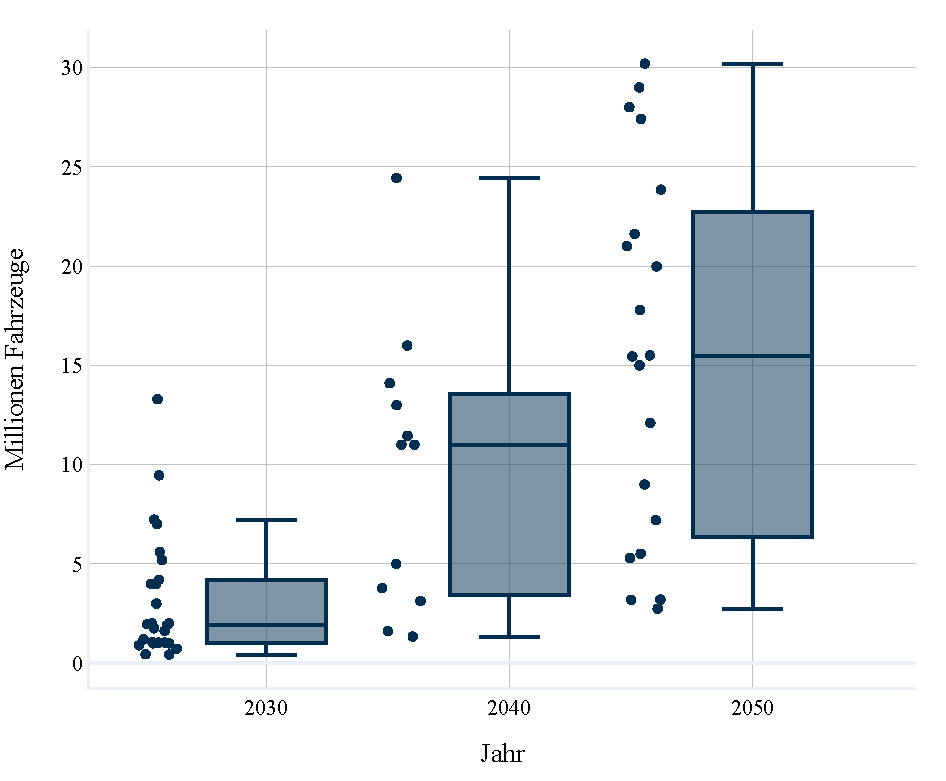
\includegraphics[width=\textwidth]{Bilder/RampUp-BEV-MA}
    \caption{Szenarienvergleich des Fahrzeugbestands von BEV bis zum Jahr \num{2050}}\label{fig:RampUpBEV}
\end{figure}

In \autoref{fig:RampUpBEV} sind die Annahmen der betrachteten Studien zum Fahrzeugbestand von \glspl{BEV} bis zum Jahr \num{2050} als Box-Plot dargestellt.
Die zugrundeliegenden Daten finden sich im Anhang in \autoref{tab:RampUpBEV}.
Trotz einer starken Streuung zeigt sich bis \num{2050} eine klare Zunahme im Bestand.
Der Median liegt 2030 noch bei \SI{1.9}{\MioStk}, steigt bis \num{2040} auf \SI{11.0}{\MioStk} und erreicht \num{2050} \SI{15.5}{\MioStk}.
Die starke Streuung lässt sich zum einen durch den unterschiedlichen Fokus der verschiedenen Studien und zum anderen durch den langen Zeithorizont und die damit verbundene Unsicherheit erklären.
Teilweise werden in einzelnen Szenarien hohe Elektrifzierungsquoten angenommen und das Einhalten des \SIrange[range-phrase=~{--}~]{80}{95}{\percent}-Ziels des Klimaschutzplans \num{2050} vorausgesetzt, während andere Szenarien eine Fortschreibung der aktuellen Entwicklungen (\gls{BAU}) untersuchen.
So handelt es sich bei dem Ausreißer im Jahr 2030 um das Elektrifizierungsszenario der dena-Leitstudie Integrierte Energiewende.
Hierbei handelt es sich um ein Szenario, welches sowohl hohe Elektrifizierungsquoten annimmt und als Leitlinie die Einhaltung des  \SIrange[range-phrase=~{--}~]{80}{95}{\percent}-Ziels setzt.\medskip

Neben dem Hochlauf an \glspl{BEV}, ist auch mit einem starken Hochlauf bei den \glspl{PHEV} zu rechnen.
Da ein Großteil der Fahrten von \glspl{PKW} eine Strecke von \SI{50}{\km} nicht überschreiten, können viele dieser Fahrten auch von \glspl{PHEV} batterieelektrisch zurückgelegt werden. \cite{Agora2019}
Unterschiede gibt es jedoch in der maximalen Ladeleistung der Fahrzeugklassen.
So werden \glspl{BEV} \num{2050} maximale Ladeleistungen von bis zu \SI{350}{\kw} aufweisen, während die maximale Ladeleistung von \glspl{PHEV} mit bis zu \SI{120}{\kw} deutlich geringer ausfällt. \cite{Kaul2019}

\begin{figure}[H]
    \centering
    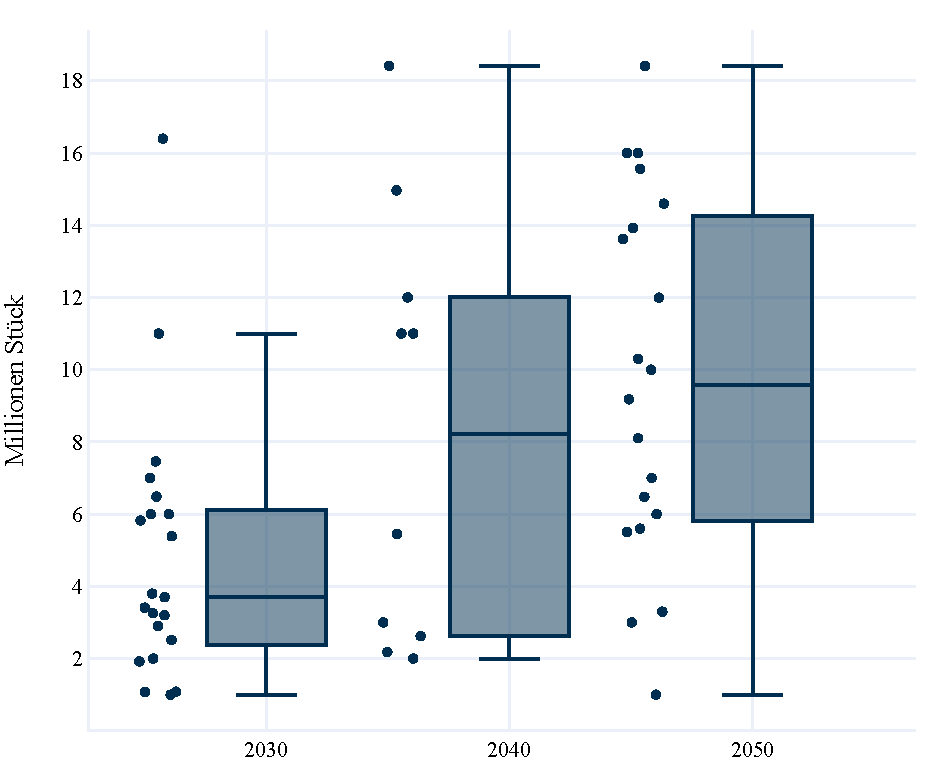
\includegraphics[width=\textwidth]{Bilder/RampUp-PHEV-MA}
    \caption{Szenarienvergleich des Fahrzeugbestands von PHEV bis zum Jahr \num{2050}}\label{fig:RampUpPHEV}
\end{figure}

\autoref{fig:RampUpPHEV} zeigt die Annahmen der betrachteten Studien zum Fahrzeugbestand von \glspl{PHEV} bis zum Jahr \num{2050} als Box-Plot.
Die zugrundeliegenden Daten finden sich im Anhang in \autoref{tab:RampUpPHEV}.
Bei \glspl{PHEV} liegt der Anstieg im Fahrzeugbestand anfangs sogar höher als bei \glspl{BEV}.
So liegt der Median 2030 bereits bei \SI{3.4}{\MioStk}.
Anschließend fällt der Fahrzeugbestand von \glspl{PHEV} hinter den der \glspl{BEV} zurück.
Bis \num{2040} steigt dieser auf \SI{8.2}{\MioStk} und \num{2050} auf \SI{9.6}{\MioStk}.
Je nach Studie und Szenario sinkt der Fahrzeugbestand nach \num{2030} sogar wieder, da unter Umständen zur Erreichung der Klimaziele der Umstieg auf \glspl{BEV} sinnvoller ist.

\begin{figure}[H]
    \centering
    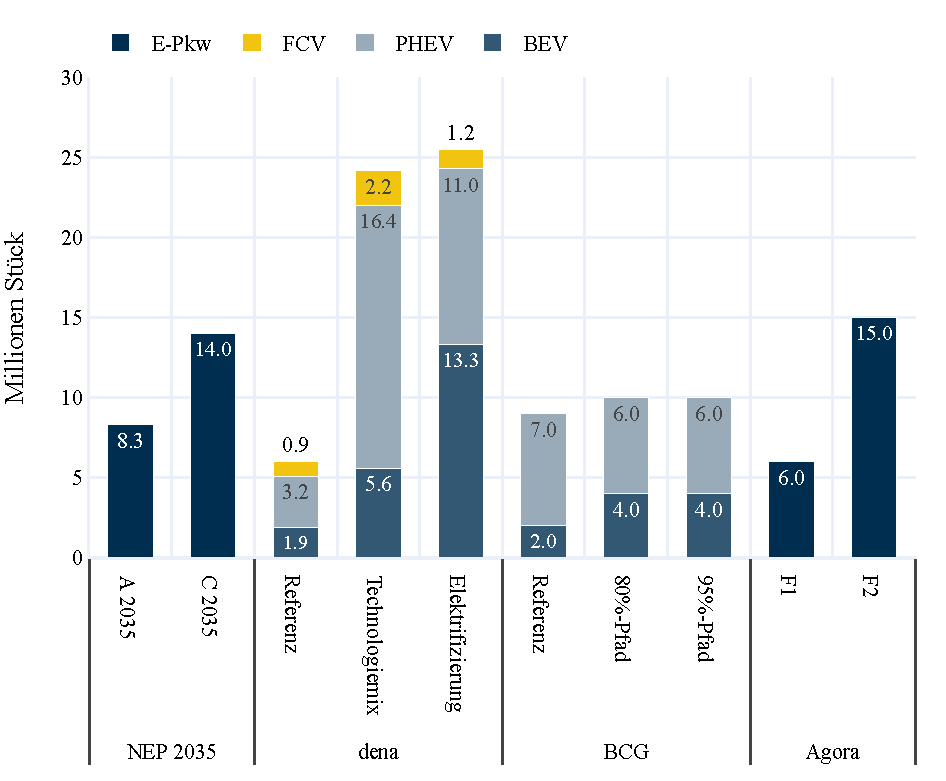
\includegraphics[width=\textwidth]{Bilder/RampUp-2030-Focus-MA}
    \caption{Fahrzeughochlauf alternativer Antriebstechnologien je Studie und Szenario bis zum Jahr \num{2030}}\label{fig:RampUp2030}
\end{figure}

Von den betrachteten Studien quantifizieren drei Studien den Netzausbaubedarf auf Verteilnetzebene und bilden somit eine Referenz zu der vorliegenden Arbeit und werden vertieft betrachtet.
Hierzu zählen die dena-Leitstudie \glqq Integrierte Energiewende\grqq{} \cite{DEAGH2018}, die BCG Studie \glqq Klimapfade für Deutschland\grqq{} \cite{BCG2018} und die Agora Studie \glqq Verteilnetzausbau für die Energiewende\grqq{} \cite{Agora2019}.
\autoref{fig:RampUp2030} zeigt den Fahrzeughochlauf verschiedener alternativer Antriebstechnologien im Verkehrssektor bis \num{2030} je Studie und Szenario.
Als Referenz wurden die konservativste und progressivste Annahmen des Netzentwicklungsplans \numrange[range-phrase=~{--}~]{2021}{2035} \cite{BNetzA2020} hinzugefügt.
Zu beachten ist hierbei, dass sich der Netzentwicklungsplan im Gegensatz zu den anderen Studien auf das Stützjahr \num{2035} bezieht.
Es wird erneut deutlich, dass sich der Markthochlauf je nach Studie und Szenario teils erheblich unterscheidet.
Grund hierfür sind nicht nur unterschiedliche Zielsetzungen der Studien, sondern auch verschiedene Modellgrundlagen und Annahmen.
So spannen sowohl die dena-Leitstudie als auch die BCG Studie einen Szenariorahmen für die Erreichung der Klimaschutzziele bis \num{2050} auf.
Dennoch liegt der Fahrzeugbestand alternativer Antriebstechnologien in den Klimaschutzszenarien \glqq Technologiemix\grqq{} und \glqq Elektrifizierung\grqq{} der dena-Leitstudie im Jahr 2030 mehr als doppelt so hoch als in den vergleichbaren Szenarien \glqq \SI{80}{\percent}-Pfad\grqq{} und \glqq \SI{95}{\percent}-Pfad\grqq{} der BCG Studie.
Beide Studien betrachten dabei die Erreichung der Klimaschutzziele über alle relevanten Sektoren.
Hierbei bewertet die BCG Studie den Verkehrssektor als deutlich unelastischer als die dena-Leitstudie, wodurch im Jahr \num{2030} eine große Diskrepanz zwischen den Szenarien entsteht.\medskip

Demgegenüber definiert die Agora Studie feste Markthochläufe und ermittelt auf Grundlage dieser den nötigen Netzausbaubedarf in Abhängigkeit verschiedener Ladestrategien und -leistungen.
Dabei basieren die angenommenen Markthochläufe in den \texttt{F}-Szenarien auf einer Fortschreibung des aktuellen Verkehrsverhaltens auf einer \glqq Antriebswende\grqq{} und in dem \texttt{M}-Szenario (s. \autoref{fig:RampUp2050}) auf einer \glqq Mobilitätswende\grqq{}.

\begin{figure}[H]
    \centering
    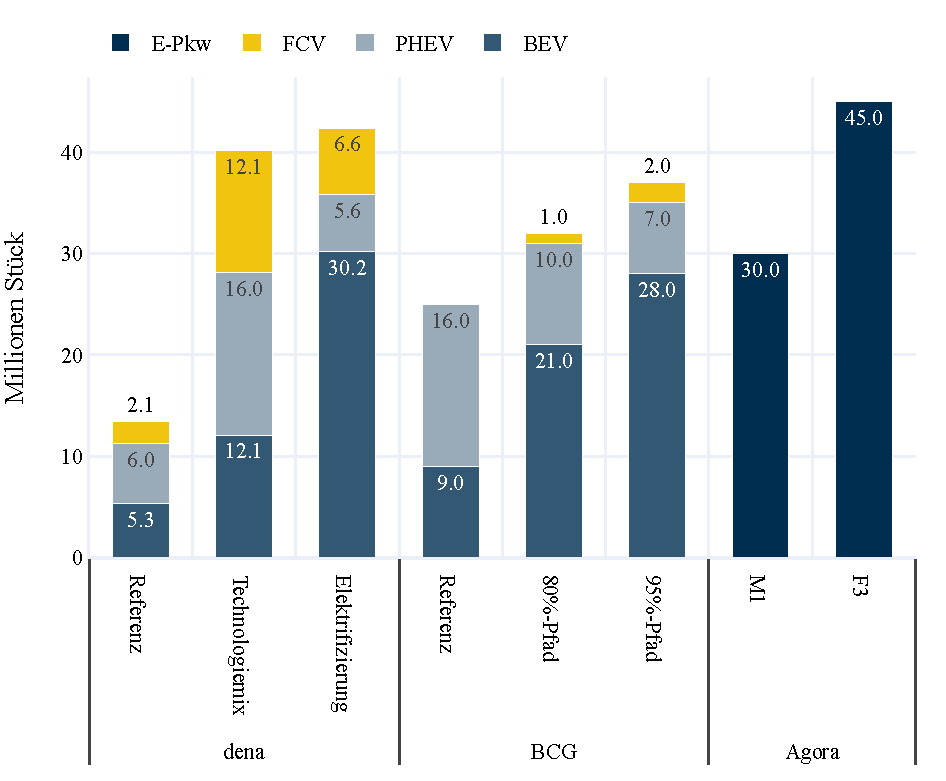
\includegraphics[width=\textwidth]{Bilder/RampUp-2050-Focus-MA}
    \caption{Fahrzeughochlauf alternativer Antriebstechnologien je Studie und Szenario bis zum Jahr \num{2050}}\label{fig:RampUp2050}
\end{figure}

In \autoref{fig:RampUp2050} findet sich der Fahrzeughochlauf verschiedener alternativer Antriebstechnologien im Verkehrssektor bis \num{2050} je Studie und Szenario.
Im Gegensatz zum Markthochlauf bis \num{2030}, liegen die Markthochlaufzahlen bis \num{2050} in allen Studien auf einem ähnlichen Niveau.
Dennoch liegen die Zahlen der BCG-Szenarien unter denen der dena-Leitstudie.
Der Grund hierfür ist, dass die Erreichung der Klimaschutzziele in der BCG Studie stärker in die Sektoren Energie, Haushalte, \gls{GHD} und Industrie verlagert werden.
Beide Studien sind sich jedoch einig, dass zum Erreichen der Klimaschutzziele der Markthochlauf von alternativer Antriebstechnologien im Verkehrssektor gegenüber dem jeweiligen Referenzszenario (\gls{BAU}) deutlich angehoben werden muss.

\subsubsection{Kosten für den Netzausbau}

Die Kosten für den Netzausbau auf Verteilnetzebene werden von drei Studien untersucht.
Hierzu zählen die dena-Leitstudie \glqq Integrierte Energiewende\grqq{} \cite{DEAGH2018}, die BCG Studie \glqq Klimapfade für Deutschland\grqq{} \cite{BCG2018} und die Agora Studie \glqq Verteilnetzausbau für die Energiewende\grqq{} \cite{Agora2019}.

\begin{figure}[H]
    \centering
    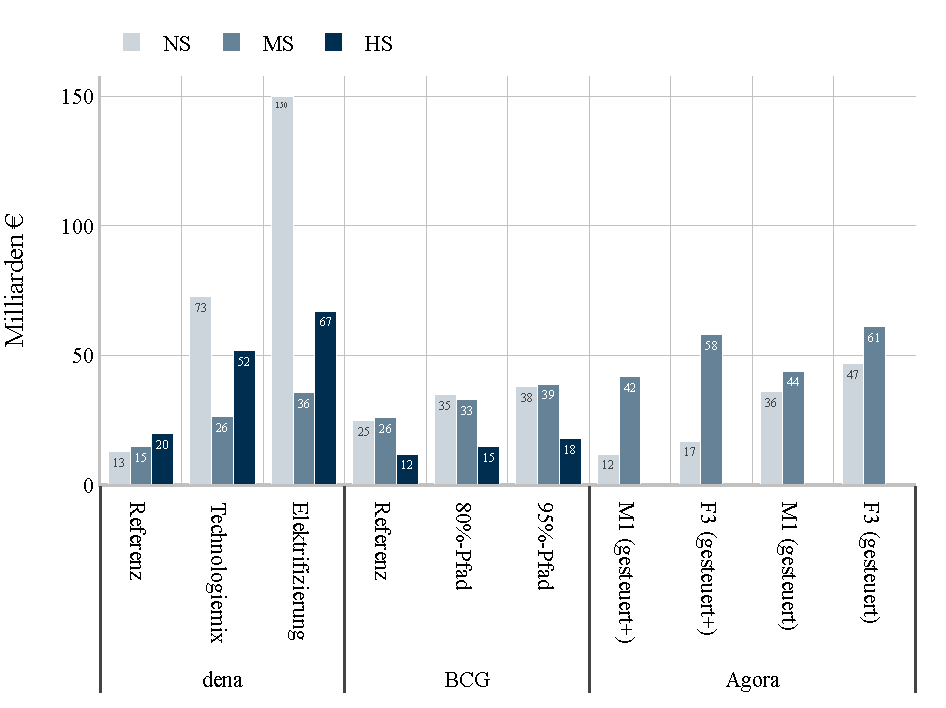
\includegraphics[width=\textwidth]{Bilder/DS-CAPEX-MA}
    \caption{Investitionsbedarf in die Verteilnetze bis zum Jahr \num{2050} je Spannungsebene}\label{fig:DSCAPEXMeta}
\end{figure}

In \autoref{fig:DSCAPEXMeta} finden sich die Ergebnisse der Studien für den Investitionsbedarf in die Verteilnetze bis zum Jahr \num{2050} aufgeteilt auf die drei Spannungsebenen \gls{NS}, \gls{MS} und \gls{HS}.
Deutlich wird hierbei, dass die dena-Leistudie die mit Abstand höchsten Kosten für den Netzausbau auf \gls{NS}- und \gls{HS}-Ebene ermittelt.
Die Agora Studie untersucht hingegen die Netzausbaukosten nicht auf der \gls{HS}-Ebene, ermittelt jedoch die höchsten Ausbaukosten auf \gls{MS}-Ebene.
Ein direkter Vergleich der Ergebnisse ist jedoch nur bedingt möglich, da die drei Studien unterschiedliche Grundsätze für ihre Szenarien und die Bestimmung des Netzausbaubedarfs ansetzen.
Deshalb sollen diese Grundsätze kurz näher betrachtet werden.

\paragraph{dena-Leitstudie \glqq Integrierte Energiewende\grqq{}:}

Ziel der dena-Leitstudie war es, Szenarien für eine Transformation des Energiesystems zur Einhaltung der Klimaschutzziele von für eine Minderung der Treibhausgasemissionen von \SIrange[range-phrase=~{--}~]{80}{95}{\percent} bis \num{2050} zu entwerfen und zu untersuchen.
Dabei wurden die Sektoren Energiewirtschaft, Gebäude, Industrie, Verkehr, Land- und
Abfallwirtschaft inkludiert.
Somit handelt es sich bei den Netzausbaukosten um die Kosten der Summe der Effekte der Umstellung aller Sektoren auf einen Klimaschutzpfad.\medskip

Neben einem Referenzszenario, welches eine progressive Fortschreibung aktueller politischer und technologischer Entwicklungen darstellt, wird zwischen Technologiemix- und Elektrifizierungsszenarien unterschieden.
Während in den Elektrifizierungsszenarien von einer hohen Elektrifizierung der Sektoren Gebäude, Industrie und Verkehr ausgegangen wird, kommt es in den Technologiemixszenarien zu einem variableren Einsatz verschiedener Technologien und Energieträger.\medskip

Die Grundlage für die Bestimmung der Netzausbaukosten bildet die Ermittlung der zukünftigen Versorgungsaufgaben in den einzelnen Netzgebieten.
Die Versorgungsaufgabe wird hierbei im wesentlichen durch den Zubau \glspl{DEA} (\glspl{PVA}, \glspl{WEA} und \glspl{BMA}), sowie neuer Lasten (\glspl{EV} und \glspl{WP}), beeinflusst.
Die Zubauprognosen erfolgen zunächst auf Bundeslandebene und werden anschließend auf Gemeindeebene verteilt.
Weiterhin erfolgt eine Einordnung der Gemeinden in \glspl{NGK} anhand ihrer Einwohnerzahl und Leistungsdichten von \glspl{EV} und \glspl{WP}.
Dies führt zu einer Clusterung der Gemeinden, wodurch das Verhalten einer Gemeinde auf das einer anderen Gemeinde übertragen werden kann.\medskip

Für die \gls{NS}- und \gls{MS}-Ebene erfolgt die Ermittlung des Netzausbaubedarfs mit Hilfe repräsentativer Netzstrukturen, welche genutzt werden um die nötigen Netzausbaumaßnahmen zu identifizieren.
Auf \gls{HS}-Ebene wird davon ausgegangen, dass der Netzausbaubedarf einen linearen Zusammenhang zum Zubau von \glspl{DEA} aufweist.
Abschließend wird der ermittelte Netzausbaubedarf auf allen Spannungsebenen monetär bewertet.\medskip

Eine Steuerung der Ladevorgänge von neuen Verbrauchern findet nicht statt.
Stattdessen geht die Studie davon aus, dass die zusätzliche Last durch \glspl{EV} und \glspl{WP} gleichzeitig mit der bisherigen Spitzenlast auftritt und der auslegungsrelevante Starklastfall somit deutlich erhöht wird.

\paragraph{BCG Studie \glqq Klimapfade für Deutschland\grqq{}:}

Auch die BCG Studie setzt sich das Erreichen der Klimaschutzziele bis \num{2050} als Ziel.
Dabei steht die volkswirtschaftliche Kosteneffizienz und die Wettbewerbsfähigkeit des Industriestandorts Deutschland im Vordergrund.
Dabei werden die gleichen Sektoren, wie in der dena-Leitstudie betrachtet. \medskip

Im Gegensatz zur dena-Leitstudie erfolgt für die Quantifizierung des Netzausbaubedarfs auf Grundlage eines vereinfachten Ansatzes.
Der Netzausbaubedarf wird in Anlehnung an die dena-Verteilnetzstudie \cite{DEAGH2012} auf Grundlage der Zubauzahlen für \glspl{DEA} und neue Verbraucher abgeschätzt und die Kosten anschließend anhand spezifischer Investitionskosten berechnet. 

{
\renewcommand{\arraystretch}{1.2}% grßerer Zeilenabstand
\sisetup{range-phrase=~{--}~}% Gedankenstrich statt "bis" bei SIrange
\begin{table}[H]
	\begin{center}
		\caption{Studienvergleich der zentralen Annahmen zur Entwicklung des Zubaus an regenerativen Erzeugungseinheiten und neuen Verbraucher bis zum Jahr \num{2050}}
		\begin{tabu} to \textwidth {X[1.5] X[1, r] X[1, r]}
			\hline
            {}                                      &   dena-Leitstudie             & BCG Studie                \\
            {}                                      &   Elektrifizierungsszenarien  & \SI{95}{\percent}-Pfad    \\\hline
            Leistung PVA in \si{\gw}                &   \num{165}                   & \num{130}                 \\
            Leistung onshore WEA in \si{\gw}        &   \num{179}                   & \num{102}                 \\
            BEV in \si{\MioStk}                     &   \num{30.2}                  & \num{28}                  \\
            PHEV in \si{\MioStk}                    &   \num{5.6}                   & \num{7}                   \\
            Wärmepumpen in \si{\MioStk}             &   \num{17}                    & \num{16}                  \\\hline
		\end{tabu}
		\label{tab:denaVSBCG}
	\end{center}
	\vspace{-3mm}%Put here to reduce too much white space after your table
\end{table}
}

\autoref{tab:denaVSBCG} zeigt die wichtigsten Annahmen der dena-Leitstudie und der BCG Studie zur Entwicklung des Zubaus an \glspl{DEA} und neuen Verbraucher bis zum Jahr \num{2050} für die jeweils progressivsten Szenarien.
Der Investitionsbedarf Die dena-Leitstudie ermittelt bis \num{2050} eine installierten Leistung von \SI{344}{\gw} an \glspl{PVA} und onshore \glspl{WEA}.
Dies ist etwa  \num{1.5}-mal so viel wie bei der BCG Studie.
Die ermittelten Zubauzahlen für die neuen Verbraucher sind hingegen bei beiden Studien ähnlich.\medskip

Dennoch ist der ermittelte Investitionsbedarf in die Verteilnetze in der dena-Leitstudie im Vergleich zur BCG Studie mehr als \num{2.5}-mal und auf \gls{NS}-Ebene sogar beinah \num{4}-mal so hoch.
Im Gegensatz zur dena-Leitstudie, wird in der BCG-Studie von einem gesteuerten Laden der neuen Verbraucher ausgegangen.
Dabei wird bei \glspl{WP} ein zweistündiger Warmwasserspeicher unterstellt, wodurch ein ebenso langer Starklastfall überbrückt werden kann.
\SI{80}{\percent} der \glspl{EV} können hingegen auf Strommarktsignale reagieren und werden nur geladen, wenn weniger als \SI{50}{\percent} des Ladestands vorhanden sind oder eine lange Fahrt ansteht.
Die starken Unterschiede im ermittelten Netzausbaubedarf sind somit sowohl eine folge der unterschiedlichen Berechnungsmethoden, der starken Differenzen im Verhalten der neuen Verbraucher als auch des unterschiedlichen starken Ausbaus an \glspl{DEA}.
Die Effekte können jedoch nicht klar differenziert werden.

\paragraph{Agora Studie \glqq Verteilnetzausbau für die Energiewende\grqq{}:}

Die Agora Studie setzt ihren Fokus ausschließlich auf die Elektromobilität und den hiermit verbundenen Netzausbaubedarf im Verteilnetz auf \gls{NS}- und \gls{MS}-Ebene.
Während die Annahmen zum Zubau von \glspl{DEA} und Wärmepumpen in den Szenarien konstant gehalten werden, wird in der Entwicklung der Elektromobilität zwischen \glqq Antriebs-\grqq{} und \glqq Mobilitätswende\grqq-Szenarien unterschieden.
Nicht elektrische Antriebstechnologien werden hierbei nicht berücksichtigt.
Zusätzlich wird ein starker Fokus auf den Einfluss von unterschiedlichen Ladestrategien auf den Netzausbaubedarf gelegt.\medskip

Die Ermittlung des Netzausbaudedarfs erfolgt analog zur Methodik der dena-Leitstudie.
Dabei wurden jedoch die Annahmen zur Gleichzeitigkeit der Ladevorgänge um eine Abhängigkeit von der Ladeleistung erweitert.
Zusätzlich wurde ein netzdienliches Ladekonzept (gesteuert) untersucht, welches eine Verschiebung der Ladevorgänge zur Residuallastglättung innerhalb der Standzeit ermöglicht, sowie ein erweitertes netzdienliches Ladekonzept (gesteuert\Plus), welches zusätzlich die Verschiebung der Ladevorgänge über mehrere Standzeiten und eine Kappung von Lastspitzen erlaubt.\medskip

Es zeigt sich, dass die Netzausbaukosten auf \gls{NS}-Ebene durch das erweiterte netzdienliche Ladekonzept deutlich gesenkt werden können, während der Einfluss auf \gls{MS}-Ebene nur gering ausfällt.
Auch zeigt sich aufgrund der Residuallastglättung des netzdienlichen Ladens im Vergleich zur dena-Leitstudie ein deutlich geringerer Netzausbaubedarf auf \gls{NS}-Ebene trotz der höheren Hochlaufzahlen an \glspl{EV} im \texttt{F3}-Szenario von \SI{45}{\MioStk} und einem vergleichbaren Ausbau an \glspl{DEA} von \SI{311}{\gw}.
Jedoch fällt der Netzausbaubedarf auf \gls{MS}-Ebene höher aus als in der dena-Leitstudie, da der Anteil an nicht steuerbaren Lasten (z.~B. Schnellladeinfrastruktur und Ladeinfrastruktur für Flotten und Busse) auf \gls{MS}-Ebene höher ausfällt und der hohe \gls{EV}-Bestand somit einen größeren Einfluss ausübt.

\subsection{Ergebnisse des Workshops \glqq Neue Verbraucher und elektrische Flexbilitäten\grqq{}}

Dieses Kapitel beschreibt und diskutiert die wichtigsten Ergebnisse des Workshops \glqq Neue Verbraucher und elektrische Flexbilitäten\grqq{}, welche die Grundlage für den Szenariorahmen bilden.
Unter Einbeziehung der Ergebnisse der Literaturrecherche aus \ref{chap:Metaanalyse} wurden verschiedene Fragestellungen im Bezug auf \glqq Neue Verbraucher und elektrische Flexbilitäten\grqq{} mit Vertretern aus Industrie, Forschung und vor allem von Netzbetreibern diskutiert.
Dabei sind für die Aufstellung des Szenariorahmens in erster Linie folgende behandelte Schwerpunkte von Bedeutung:

\begin{itemize}
    \item Elektromobilitätsszenarien
    \item Elektrische Flexibilitäten
    \item Neue Verbraucher in der Verteilnetzplanung
\end{itemize}

\paragraph{Elektromobilitätsszenarien:}

%ToDo!: Welche Jahreszahl als Stütztjahr, oder stattdessen nur eine Hochlaufzahl?

Bei dem Schwerpunkt \glqq Elektromobilitätsszenarien\grqq{} stand die Aufstellung eines groben Szenariorahmens für den Hochlauf an \glspl{EV} im Vordergrund.
Dabei wurden folgende Szeanriorahmen diskutiert und es wurde darüber abgestimmt, welche Szenariorahmen von besonderem Interesse sind:

\begin{itemize}
    \item Mobilitätswende
    \item Klimaschutz
    \item Antriebswende (Vollelektrifizierung)
\end{itemize}

Bei der Abstimmung wurde deutlich, dass vor allem ein Mobilitätswende-Szenario von großem Interesse für die Teilnehmer des Workshops ist.
Um mit dieser Arbeit einen möglichst breiten Horizont abzudecken, werden somit neben einem Referenzszenario ein Mobilitätswende-Szenario mit verhältnismäßig geringem Anteil an \glspl{MIV} und ein Antriebswende-Szenario mit einem hohen Anteil an \glspl{MIV} betrachtet.\medskip

Bei der Ladeinfrastruktur stellte sich heraus, dass erwartet wird, dass vor allem die große Anzahl an \gls{AC}-Ladepunkten mit niedrigen Ladeleistungen und einer hohen Gleichzeitigkeit im privaten Bereich und am Arbeitsplatz zu Problemen führen wird.
Regionale Konzentrationen von Ladepunkten und somit eine regional stark unterschieldiche Netzbelastung sind hingegen nur bei geringen Durchdringungen der Elektromobilität von Bedeutung und zu erwarten.

\paragraph{Elektrische Flexibilitäten:}

% Definition zeitlich und räumlich
% V2G hat vermutlich keine Zukunft

\paragraph{Neue Verbraucher in der Verteilnetzplanung:}

\subsection{Annahmen}

\subsubsection{Ausbau regenerativer Energien}

\subsubsection{Wärmepumpen}

\subsubsection{Elektromobilität}

Bei der Elektromobilität müssen neben Annahmen zu den Zahlen zum Fahrzeughochlauf auch die technischen Daten der Fahrzeuge und der Ladeinfrastruktur berücksichtigt werden.

\paragraph{Fahrzeughochlauf:}
Der Fahrzeughochlauf unterscheidet sich je nach Szenario.
Für das Stützjahr \num{2035} wird nur ein Szenario untersucht, wobei der Fahrzeughochlauf mit \SI{14}{\MioStk} den Annahmen des Szenarios C~\num{2035} des Netzentwicklungsplans \numrange[range-phrase=~{--}~]{2021}{2035} \cite{BNetzA2020} entspricht.
Die Hochlaufzahlen für das Referenzszenario entsprechen mit \SI{25.1}{\MioStk} den summierten Medianen der Literaturrecherche für den Fahrzeughochlauf an \glspl{BEV} und \glspl{PHEV}.
Beim Mobilitätswende-Szenario wurde der Fahrzeugbestand des Effizienz-Plus Szenarios des Renewbility~III Projekts \cite{Institut2016} übernommen und von einer vollständigen Elektrifizierung ausgegangen.
Das Antriebswende-Szenario spiegelt hingegen den Fahrzeugbestand von \SI{47.7}{\MioStk} vom \DTMdate{2020-01-01} \cite{KBA2020} wieder.

{
\renewcommand{\arraystretch}{1.2}% grßerer Zeilenabstand
\sisetup{range-phrase=~{--}~}% Gedankenstrich statt "bis" bei SIrange
\begin{table}[H]
	\begin{center}
		\caption{Hochlaufzahlen für E-Pkw je Szenario}
		\begin{tabu} to \textwidth {X[1.2] X[0.8, r] X[1, r] X[1, r] X[1, r]}
            \hline
                                    & \num{2035}           & \multicolumn{3}{c}{\num{2050}}                            \\
                                    &                      & Referenz          & Mobilitätswende   & Antriebswende     \\ \hline
            E-Pkw in \si{\MioStkSC} & \num{14.0}           & \num{25.1}        & \num{37.7}        & \num{47.7}        \\
            BEV Kleinwagen          & \SI{13}{\percent}    & \SI{16}{\percent} & \SI{38}{\percent} & \SI{16}{\percent} \\
            BEV Mittelklasse        & \SI{30}{\percent}    & \SI{35}{\percent} & \SI{26}{\percent} & \SI{35}{\percent} \\
            BEV Oberklasse          & \SI{9}{\percent}     & \SI{11}{\percent} & \SI{11}{\percent} & \SI{11}{\percent} \\
            PHEV Kleinwagen         & \SI{12}{\percent}    & \SI{10}{\percent} & \SI{13}{\percent} & \SI{10}{\percent} \\
            PHEV Mittelklasse       & \SI{27}{\percent}    & \SI{22}{\percent} & \SI{9}{\percent}  & \SI{22}{\percent} \\
            PHEV Oberklasse         & \SI{8}{\percent}     & \SI{7}{\percent}  & \SI{4}{\percent}  & \SI{7}{\percent}  \\ \hline
		\end{tabu}
		\label{tab:SzenarienRampUp}
	\end{center}
	\vspace{-3mm}%Put here to reduce too much white space after your table
\end{table}
}

Die Aufteilung in \glspl{BEV} und \glspl{PHEV} erfolgt für das Stütztjahr \num{2035}, sowie das Referenz- und Antriebswende-Szenario anhand der ermittelten Mediane der Literaturrecherche für den Fahrzeughochlauf an \glspl{BEV} und \glspl{PHEV} für das jeweilige Jahr.
Für das Jahr \num{2035} erfolgt eine lineare Interpolation zwischen den Jahren \num{2030} und \num{2040}.
Im Mobilitätswende-Szenario wird hingegen davon ausgegangen, dass sich der Anteil an vollständig elektrifizierten Fahrzeugen erhöht.
Der Anteil an \glspl{BEV} entspricht in diesem Szenario \SI{75}{\percent}, wodurch der Anteil an \glspl{PHEV} auf \SI{25}{\percent} sinkt.\medskip

Innerhalb der Fahrzeugtypen erfolgt weiterhin eine Einteilung in die Fahrzeugklassen Kleinwagen, Mittelklasse und Oberklasse.
Es wird davon ausgegangen, dass sich die Einteilung zwischen \glspl{BEV} und \glspl{PHEV} nicht unterscheidet.
Für das Stütztjahr \num{2035}, sowie das Referenz- und Antriebswende-Szenario entspricht die Einteilung der Statistik des Kraftfahrt-Bundesamtes \cite{KBASegments2020} vom \DTMdate{2020-01-01}.
Es wird somit von einer Fortschreibung des aktuellen Verbraucherverhaltens ausgegangen.
Eine genaue Zuordnung der \gls{PKW}-Segmente in die Klassen findet sich im Anhang (\autoref{tab:KBASegments} und \autoref{tab:Segments}).
Im Mobilitätswende-Szenario wird hingegen davon ausgegangen, dass es durch ein erhöhtes Umweltbewusstsein der Verbraucher zu einer Verschiebung der Anteile der Klassen kommt.
In diesem Szenario entfallen \SI{50}{\percent} aller Fahrzeuge in die Kleinwagen-Klasse, \SI{35}{\percent} in die Mittelklasse und nur \SI{15}{\percent} in die Oberklasse.

\paragraph{Technische Daten:}

Die technischen Daten der Fahrzeuge sind klassenspezifisch und innerhalb ihrer Klasse homogen.
In \autoref{tab:TechPowerCap} finden sich die fahrzeugseitige maximale Ladeleistung und die nutzbare Batteriekapazität der jeweiligen Fahrzeugklassen.
Eine Limitierung der Ladeleistung durch die Unterscheidung in Normal- und Schnellladung, erfolgt im Simulationsmodell von Seiten der Ladeinfrastruktur.

{
\renewcommand{\arraystretch}{1.2}% grßerer Zeilenabstand
\sisetup{range-phrase=~{--}~}% Gedankenstrich statt "bis" bei SIrange
\begin{table}[H]
	\begin{center}
		\caption{Maximale Ladeleistung und nutzbare Batteriekapazität je Fahrzeugklasse}
		\begin{tabu} to \textwidth {X[1.2] X[1, r] X[1, r] X[1, r] X[1, r]}
            \hline
                              & \multicolumn{2}{c}{Ladeleistung in \si{\kw}} & \multicolumn{2}{c}{Batteriekapazität in \si{\kwh}} \\
            Fahrzeugklasse    & \num{2035}                & \num{2050}                & \num{2035}                   & \num{2050}                   \\ \hline
            BEV Kleinwagen    & \num{120}                 & \num{120}                 & \num{60}                     & \num{70}                     \\
            BEV Mittelklasse  & \num{350}                 & \num{350}                 & \num{90}                     & \num{100}                    \\
            BEV Oberklasse    & \num{350}                 & \num{350}                 & \num{110}                    & \num{120}                    \\
            PHEV Kleinwagen   & \num{40}                  & \num{120}                 & \num{14}                     & \num{25}                     \\
            PHEV Mittelklasse & \num{40}                  & \num{120}                 & \num{20}                     & \num{30}                     \\
            PHEV Oberklasse   & \num{120}                 & \num{120}                 & \num{30}                     & \num{40}                     \\ \hline
            \multicolumn{5}{l}{Quelle: Szenario \glqq Verstärkte Elektrifizierung\grqq{} \cite{Kaul2019}}
		\end{tabu}
		\label{tab:TechPowerCap}
	\end{center}
	\vspace{-3mm}%Put here to reduce too much white space after your table
\end{table}
}

Der elektrische Energieverbrauch der Fahrzeuge wird aus den Annahmen der Studie \glqq eMobil \num{2050}\grqq{} \cite{Hacker2014} abgeleitet.
Es wird angenommen, dass Kleinwagen gegenüber Mittelklasse Fahrzeugen einen um \SI{20}{\percent} reduzierten Energieverbrauch aufweisen.
Oberklasse Fahrzeuge weisen hingegen einen um \SI{20}{\percent} erhöhten Energieverbrauch auf.\medskip

Für das Jahr \num{2035} erfolgt eine lineare Interpolation zwischen den Verbrauchswerten von \num{2030} und \num{2040}.
Weiterhin bietet die Studie \glqq eMobil \num{2050}\grqq{} nur Verbrauchsangaben nach dem \glspl{NEFZ}, welche nicht realen Verbrauchsdaten entsprechen.
Nach \cite{Heinfellner2015} lag der Realverbrauch \num{2013} gegenüber einer Messung nach \gls{NEFZ} im Mittel um \SI{27}{\percent} höher.
Die Werte der Studie \glqq eMobil \num{2050}\grqq{} wurden um diesen Faktor erhöht.

{
\renewcommand{\arraystretch}{1.2}% grßerer Zeilenabstand
\sisetup{range-phrase=~{--}~}% Gedankenstrich statt "bis" bei SIrange
\begin{table}[H]
	\begin{center}
		\caption{Durchschnittlicher elektrischer Energieverbrauch je Fahrzeugklasse}
		\begin{tabu} to \textwidth {X[1] X[1, r] X[1, r]}
            \hline
                              & \multicolumn{2}{c}{Verbrauch in \si{\kwhkm}}  \\
            Fahrzeugklasse    & \num{2035}            & \num{2050}            \\ \hline
            BEV Kleinwagen    & \num{14.0}            & \num{11.9}            \\
            BEV Mittelklasse  & \num{17.5}            & \num{14.8}            \\
            BEV Oberklasse    & \num{21.0}            & \num{17.8}            \\
            PHEV Kleinwagen   & \num{14.3}            & \num{12.1}            \\
            PHEV Mittelklasse & \num{17.8}            & \num{15.2}            \\
            PHEV Oberklasse   & \num{21.4}            & \num{18.2}            \\ \hline
		\end{tabu}
		\label{tab:TechVerbrauch}
	\end{center}
	\vspace{-3mm}%Put here to reduce too much white space after your table
\end{table}
}

\paragraph{Ladeinfrastruktur:}

Die Ladeinfrastruktur wird im Gegensatz zu den Annahmen zum Fahrzeughochlauf nicht in absoluten Zahlen ausgedrückt.
Stattdessen werden den einzelnen Wegezwecken der Fahrzeuge Wahrscheinlichkeiten zugeordnet, dass das Fahrzeug am Zielort geladen werden kann.
Weiterhin wird diese Wahrscheinlichkeit auf verschiedene Ladeleistungen aufgeteilt.
Dabei wird grundsätzlich zwischen Normal- und Schnellladung unterschieden.
Normalladung beschreibt in dieser Masterarbeit alle Ladevorgänge mit einer Leistung von bis zu einschließlich \SI{50}{\kw} und Schnellladung alle Ladevorgänge von größer \SIrange[range-phrase=~bis~einschließlich~]{50}{350}{\kw}.

\subparagraph{Normalladung} beinhaltet in dieser Arbeit die Leistungsklassen \SI{3.7}{\kw}, \SI{11}{\kw}, \SI{22}{\kw} und \SI{50}{\kw}.
Eine Zuordnung der Leistungsklassen auf die einzelnen Wegezwecke erfordert vorerst eine Zuordnung der \UCs auf die Wegezwecke.
In \autoref{tab:WegLadeUseCase} findet sich die entsprechende prozentuale Aufteilung der \UCs auf die Wegezwecke.

{
\renewcommand{\arraystretch}{1.2}% grßerer Zeilenabstand
\sisetup{range-phrase=~{--}~}% Gedankenstrich statt "bis" bei SIrange
\begin{table}[H]
	\begin{center}
		\caption{Prozentuale Zuordnung der \UCs auf die verschiedenen Wegezwecke}
		\begin{tabu} to \textwidth {X[1.2] X[1.1, r] X[1.3, r] X[1.7, r] X[1.8, r] X[1.2, r]}
            \hline
            Wegezweck  & Eigenheim           & Wohnanlage          & Firmenparkplatz     & Gewerbeparkplatz   & Straßenrand         \\ \hline
            Arbeit     & \SI{0.0}{\percent}  & \SI{0.0}{\percent}  & \SI{64.5}{\percent} & \SI{0.0}{\percent}  & \SI{35.5}{\percent} \\
            dienstlich & \SI{0.0}{\percent}  & \SI{0.0}{\percent}  & \SI{38.0}{\percent} & \SI{6.0}{\percent}  & \SI{56.0}{\percent} \\
            Ausbildung & \SI{0.0}{\percent}  & \SI{0.0}{\percent}  & \SI{64.5}{\percent} & \SI{0.0}{\percent}  & \SI{35.5}{\percent} \\
            Einkauf    & \SI{0.0}{\percent}  & \SI{0.0}{\percent}  & \SI{0.0}{\percent}  & \SI{76.5}{\percent} & \SI{23.5}{\percent} \\
            Erledigung & \SI{0.0}{\percent}  & \SI{0.0}{\percent}  & \SI{0.0}{\percent}  & \SI{38.0}{\percent} & \SI{62.0}{\percent} \\
            Freizeit   & \SI{0.0}{\percent}  & \SI{0.0}{\percent}  & \SI{0.0}{\percent}  & \SI{38.5}{\percent} & \SI{61.5}{\percent} \\
            nach Hause & \SI{43.4}{\percent} & \SI{25.1}{\percent} & \SI{0.0}{\percent}  & \SI{0.0}{\percent}  & \SI{31.4}{\percent} \\ \hline
		\end{tabu}
		\label{tab:WegLadeUseCase}
	\end{center}
	\vspace{-3mm}%Put here to reduce too much white space after your table
\end{table}
}

Derzeit leben in Deutschland ungefähr \SI{44.2}{\MioMen} in Gebäuden mit maximal zwei Wohnungen und \SI{37.2}{\MioMen} in Mehrfamilienhäusern.
Etwa \SI{80}{\percent} der Fahrzeugbesitzer in Gebäuden mit maximal zwei Wohnungen verfügen über einen Stellplatz in der Garage oder im \texttt{Carport}.
In Mehrfamilienhäusern haben hingegen nur \SI{55}{\percent} der Fahrzeugbesitzer einen Stellplatz. \cite{dena2020}
Unter der vereinfachenden Annahme einer gleichmäßigen Verteilung von Fahrzeugen zwischen Bewohnern von Ein- und Mehrfamilienhäusern ergibt sich hieraus die ermittelte Aufteilung der \UCs auf den Wegezweck \nHdot.\medskip

Die Aufteilung der \UCs auf die Wegezwecke \Einkaufdot, \Erledigung und \Freizeitdot, ergeben sich aus den Wegeanteilen nach Fahrtzweck im \gls{MIV}-Privatverkehr. \cite{Rikus2015}
Im Falle des Wegezwecks \Einkaufdot, wird angenommen, dass Lebensmittelgschäfte einen Gewerbeparkplatz für jeden Kunden vorhalten. Weiterhin wird angenommen, dass im Falle von sonstigen Waren und sonstigen Dienstleistungen in \SI{50}{\percent} der Fälle ein Gewerbeparkplatz zur Verfügung steht.
Bei dem Wegezweck \Erledigungdot, wird davon ausgegangen, dass beim Besuch von Behörden, Banken, Post und Geldautomaten ein Gewerbeparkplatz vorhanden ist und bei sonstigen Erledigungen in \SI{50}{\percent} der Fälle.
Für den Wegezweck \Freizeitdot, wird angenommen, dass bei kulturelle Einrichtungen und Veranstaltungen ein Gewerbeparkplatz vorhanden ist.
Bei sonstigen Freizeitaktivitäten wird angenommen, dass in \SI{50}{\percent} der Fälle ein Gewerbeparkplatz vorhanden ist.
In allen verbleibenden Fällen erfolgt ein Parken am Straßenrand.\medskip

Für die Abschätzung der Wahrscheinlichkeit auf einem Firmenparkplatz für den Wegezweck \Arbeit parken zu können, wurde die Parkplatzsituation am Arbeitsplatz zugrunde gelegt.
Demnach werden \SI{67}{\percent} aller Arbeitswege mit dem \gls{PKW} zurückgelegt, wenn die Parkplatzsituation als nicht schwierig eingestuft wird.
Demgegenüber werden bei einer schwierigen Parkplatzsituation nur \SI{36}{\percent} der Arbeitswege mit dem \gls{PKW} zurückgelegt.
Insgesamt werden mit dem \gls{PKW} \SI{56}{\percent} aller Arbeitswege zurückgelegt. \cite{Ecke2020}
Unter der Annahme, dass eine nicht schwierige Parkplatzsituation am Arbeitsplatz gleichbedeutend mit einem Firmenparkplatz und eine schwierige Parkplatzsituation mit dem Parken am Straßenrand ist, ergeben sich hieraus die ermittelten Anteile für den Wegezweck \Arbeitdot.
Weiterhin wird angenommen, dass dieses Verhältnis auf den Wegezweck \Ausbildung~übertragen werden kann.\medskip

Für den Wegezweck \dienstdot, wird die Aufteilung nach dem üblichen Stellplatz am Fahrtziel im Wirtschaftsverkehr verwendet. \cite{Rikus2015}
Demnach parken gewerbliche Halter im Wirtschaftsverkehr in \SI{30}{\percent} der Fälle am Straßenrand.
In \SI{26}{\percent} der Fälle erfolgt das Parken auf einem Privatgrundstück.
Im Wirtschaftsverkehr handelt es sich in der Regel nicht um das eigene Privatgrundstück, weswegen diese Art des Parkens ebenfalls als Parken am Straßenrand gewertet wird.
In \SI{6}{\percent} der Fälle erfolgt das Parken auf einem Gewerbeparkplatz und in \SI{38}{\percent} der Fälle auf einem Firmenparkplatz.\medskip

Anschließend erfolgt für die Stützjahre \num{2035} und \num{2050} je \UC eine Abschätzung der Wahrscheinlichkeiten, ob eine Ladung stattfinden kann und mit welcher Ladeleistung geladen werden kann.
In \autoref{tab:UCProbability2035} und \autoref{tab:UCProbability2050} die entsprechenden Annahmen.

{
\renewcommand{\arraystretch}{1.2}% grßerer Zeilenabstand
\sisetup{range-phrase=~{--}~}% Gedankenstrich statt "bis" bei SIrange
\begin{table}[H]
	\begin{center}
		\caption{Wahrscheinlichkeitverteilung der Ladeleistungen je \UC für das Stützjahr \num{2035}}
		\begin{tabu} to \textwidth {X[1.7] X[1.3, r] X[1, r] X[1, r] X[1, r] X[1, r]}
            \hline
            Lade Use   Case   & keine Ladung        & \SI{3.7}{\kw}       & \SI{11}{\kw}        & \SI{22}{\kw}        & \SI{50}{\kw}        \\ \hline
            Eigenheim         & \SI{15.0}{\percent} & \SI{17.0}{\percent} & \SI{59.5}{\percent} & \SI{8.5}{\percent}  & \SI{0.0}{\percent}  \\
            Wohnanlage        & \SI{75.0}{\percent} & \SI{3.8}{\percent}  & \SI{20.0}{\percent} & \SI{1.3}{\percent}  & \SI{0.0}{\percent}  \\
            Firmenparkplatz   & \SI{50.0}{\percent} & \SI{5.0}{\percent}  & \SI{5.0}{\percent}  & \SI{30.0}{\percent} & \SI{10.0}{\percent} \\
            Gewerbeparkplatz  & \SI{50.0}{\percent} & \SI{0.0}{\percent}  & \SI{5.0}{\percent}  & \SI{30.0}{\percent} & \SI{15.0}{\percent} \\
            Straßenrand       & \SI{75.0}{\percent} & \SI{2.5}{\percent}  & \SI{2.5}{\percent}  & \SI{15.0}{\percent} & \SI{5.0}{\percent}  \\ \hline
		\end{tabu}
		\label{tab:UCProbability2035}
	\end{center}
	\vspace{-3mm}%Put here to reduce too much white space after your table
\end{table}
}

{
\renewcommand{\arraystretch}{1.2}% grßerer Zeilenabstand
\sisetup{range-phrase=~{--}~}% Gedankenstrich statt "bis" bei SIrange
\begin{table}[H]
	\begin{center}
		\caption{Wahrscheinlichkeitverteilung der Ladeleistungen je \UC für das Stützjahr \num{2050}}
		\begin{tabu} to \textwidth {X[1.7] X[1.3, r] X[1, r] X[1, r] X[1, r] X[1, r]}
            \hline
            Lade Use   Case  & keine Ladung        & \SI{3.7}{\kw}      & \SI{11}{\kw}        & \SI{22}{\kw}        & \SI{50}{\kw}        \\ \hline
            Eigenheim        & \SI{0.0}{\percent}  & \SI{0.0}{\percent} & \SI{75.0}{\percent} & \SI{25.0}{\percent} & \SI{0.0}{\percent}  \\
            Wohnanlage       & \SI{25.0}{\percent} & \SI{7.5}{\percent} & \SI{60.0}{\percent} & \SI{7.5}{\percent}  & \SI{0.0}{\percent}  \\
            Firmenparkplatz  & \SI{25.0}{\percent} & \SI{0.0}{\percent} & \SI{7.5}{\percent}  & \SI{48.8}{\percent} & \SI{18.8}{\percent} \\
            Gewerbeparkplatz & \SI{25.0}{\percent} & \SI{0.0}{\percent} & \SI{7.5}{\percent}  & \SI{45.0}{\percent} & \SI{22.5}{\percent} \\
            Straßenrand      & \SI{50.0}{\percent} & \SI{0.0}{\percent} & \SI{5.0}{\percent}  & \SI{32.5}{\percent} & \SI{12.5}{\percent} \\ \hline
		\end{tabu}
		\label{tab:UCProbability2050}
	\end{center}
	\vspace{-3mm}%Put here to reduce too much white space after your table
\end{table}
}

In allen \UCs wird davon ausgegangen, dass die Ladevorgänge mit der Zeit mit immer höheren Ladeleistungen stattfinden werden.
Für den \UC \Eigenheim wird angenommen, dass jeder Besitzer eines \gls{EPKW} eine Ladevorrichtung vorhält, wenn die technischen Vorraussetzungen gegeben sind.
Bei rund \SI{15}{\percent} der Stellplätze der Gebäude mit einer oder zwei Wohnungen besteht kein Zugang zum Stromnetz. \cite{dena2020}
Es wird angenommen, dass dieser Bestand bis \num{2035} bestehen bleibt.
Bis \num{2050} wird hingegen davon ausgegangen, dass alle Stellplätze mit einem Netzanschluss ausgerüstet werden.
Die Aufteilung der Ladeleistungen erfolgt in Anlehnung an \cite{NPZMAVE2020}.
Dabei wird der Anteil von Ladevorgängen mit \SI{3.7}{\kw} bis \num{2035} weiter abnehmen und \num{2050} keine Rolle mehr spielen.
Der Anteil an Ladevorgängen mit \SI{11}{\kw} wird weiter wachsen, allerdings langsamer als der Anteil an Ladevorgängen mit \SI{22}{\kw}.
Eine Ladung mit \SI{50}{\kw} wird im privaten Bereich keine Rolle spielen.
\num{2035} beträgt das Verhältnis zwischen den Ladeleistungen \(20:70:10:0\) und verschiebt sich bis \num{2050} auf \(0:75:25:0\)\medskip

Stellplätze von Mehrfamilienhäusern besitzen mit ungefähr \SI{50}{\percent} deutlich seltener Zugang zum Stromnetz. \cite{dena2020}
Zusätzlich wird angenommen, dass bis \num{2035} nur die Hälfte aller Stellplätze mit Netzanschluss mit einer Ladevorrichtung ausgestattet werden.
In \num{2050} werden \SI{75}{\percent} der Stellplätze mit einem Netzanschluss ausgestattet sein und es wird angenommen, dass alle Stellplätze mit den entsprechenden technischen Vorraussetzungen mit einer Ladevorrichtung ausgestattet werden.
In Wohnanlagen werden hohe Ladeleistungen eine Ausnahme bleiben.
In \num{2035} wird von einem Verhältnis der Ladeleistungen von \(15:80:5:0\) ausgegangen, welches sich bis \num{2050} auf \(10:80:10:0\) verschiebt.\medskip

Bei Firmen- und Gewerbeparkplätzen wird von einer ähnlichen Entwicklung Ausgegangen.
Bis \num{2035} werden Mitarbeiter bzw. Kunden in \SI{50}{\percent} der Fälle Zugriff auf einen Ladepunkt haben.
Dieser Anteil steigt bis \num{2050} auf \SI{75}{\percent}.
Die Verteilung der Ladeleistungen geschieht in Anlehnung an das Ladesäulenregister der Bundesnetzagentur \cite[][Stand: \DTMdate{2020-09-09}]{BundesnetzagenturElektrizitaet2020} und der Stromtankstellen Statistik des \texttt{GoingElectric} Forums \cite[][Stand: \DTMdate{2020-10-21}]{Weemaes2020}.
Demnach besitzt ein Großteil (\SIrange[range-phrase=~bzw.~]{80}{51}{\percent}) der öffentlich zugänglichen Ladepunkte eine Ladeleistung von \SIrange{22}{42}{\kw}.
Es wird davon ausgegangen, dass sich der Trend zu hohen Ladeleistungen weiter fortsetzt.
Dies gilt jedoch vor allem für Gewerbeparkplätze, da hohe Ladeleistungen und die Verfügbarkeit von Ladepunkten zur Kundenakquise genutzt werden.
Bei Firmenparkplätzen wird \num{2035} mit einem Verhältnis von \(10:40:40:10\) gerechnet und \num{2050} von \(0:40:40:20\).
Demgegenüber wird bei Gewerbeparkplätzen \num{2035} und \num{2050} mit einem Verhältnis von \(0:10:60:30\) gerechnet.\medskip

Im Falle des \UCs \Straszenranddot, wird angenommen, dass \num{2035} noch in \SI{75}{\percent} der Fälle kein Ladepunkt zur Verfügung steht.
Dieser Anteil sinkt bis \num{2050} auf \SI{50}{\percent}.
Weiterhin entspricht das Verhältnis der Ladeleistungen dem der Firmenparkplätze mit moderateren Ladeleistungen.\medskip

Aus den zuvor getroffenen Annahmen können nun die Wahrscheinlichkeiten für die Ladevorgänge je Wegezweck berechnet werden. Die entsprechenden Ergebnisse finden sich in \autoref{tab:WegezweckProbability2035} und \autoref{tab:WegezweckProbability2050}.

{
\renewcommand{\arraystretch}{1.2}% grßerer Zeilenabstand
\sisetup{range-phrase=~{--}~}% Gedankenstrich statt "bis" bei SIrange
\begin{table}[H]
	\begin{center}
		\caption{Wahrscheinlichkeitverteilung der Ladeleistungen je Wegezweck für das Stützjahr \num{2035}}
		\begin{tabu} to \textwidth {X[1.2] X[1.2, r] X[1, r] X[1, r] X[1, r] X[1, r]}
			\hline
			Wegezweck  & keine Ladung        & \SI{3.7}{\kw}      & \SI{11}{\kw}        & \SI{22}{\kw}        & \SI{50}{\kw}        \\ \hline
			Arbeit     & \SI{58.9}{\percent} & \SI{4.1}{\percent} & \SI{16.5}{\percent} & \SI{16.5}{\percent} & \SI{4.1}{\percent}  \\
			dienstlich & \SI{64.0}{\percent} & \SI{3.3}{\percent} & \SI{13.5}{\percent} & \SI{15.0}{\percent} & \SI{4.2}{\percent}  \\
			Ausbildung & \SI{58.9}{\percent} & \SI{4.1}{\percent} & \SI{16.5}{\percent} & \SI{16.5}{\percent} & \SI{4.1}{\percent}  \\
			Einkauf    & \SI{55.9}{\percent} & \SI{0.6}{\percent} & \SI{6.2}{\percent}  & \SI{25.3}{\percent} & \SI{12.1}{\percent} \\
			Erledigung & \SI{65.5}{\percent} & \SI{1.6}{\percent} & \SI{8.1}{\percent}  & \SI{17.6}{\percent} & \SI{7.3}{\percent}  \\
			Freizeit   & \SI{65.4}{\percent} & \SI{1.5}{\percent} & \SI{8.1}{\percent}  & \SI{17.7}{\percent} & \SI{7.3}{\percent}  \\
			nach Hause & \SI{48.9}{\percent} & \SI{9.1}{\percent} & \SI{34.0}{\percent} & \SI{7.1}{\percent}  & \SI{0.8}{\percent}  \\ \hline
		\end{tabu}
		\label{tab:WegezweckProbability2035}
	\end{center}
	\vspace{-3mm}%Put here to reduce too much white space after your table
\end{table}
}

{
\renewcommand{\arraystretch}{1.2}% grßerer Zeilenabstand
\sisetup{range-phrase=~{--}~}% Gedankenstrich statt "bis" bei SIrange
\begin{table}[H]
	\begin{center}
		\caption{Wahrscheinlichkeitverteilung der Ladeleistungen je Wegezweck für das Stützjahr \num{2050}}
		\begin{tabu} to \textwidth {X[1.2] X[1.2, r] X[1, r] X[1, r] X[1, r] X[1, r]}
			\hline
			Wegezweck  & keine Ladung        & \SI{3.7}{\kw}      & \SI{11}{\kw}        & \SI{22}{\kw}        & \SI{50}{\kw}        \\ \hline
			Arbeit     & \SI{33.9}{\percent} & \SI{0.0}{\percent} & \SI{26.5}{\percent} & \SI{26.5}{\percent} & \SI{13.2}{\percent} \\
			dienstlich & \SI{39.0}{\percent} & \SI{0.0}{\percent} & \SI{23.1}{\percent} & \SI{25.3}{\percent} & \SI{12.7}{\percent} \\
			Ausbildung & \SI{33.9}{\percent} & \SI{0.0}{\percent} & \SI{26.5}{\percent} & \SI{26.5}{\percent} & \SI{13.2}{\percent} \\
			Einkauf    & \SI{30.9}{\percent} & \SI{0.0}{\percent} & \SI{10.4}{\percent} & \SI{39.1}{\percent} & \SI{19.6}{\percent} \\
			Erledigung & \SI{40.5}{\percent} & \SI{0.0}{\percent} & \SI{15.3}{\percent} & \SI{29.5}{\percent} & \SI{14.8}{\percent} \\
			Freizeit   & \SI{40.4}{\percent} & \SI{0.0}{\percent} & \SI{15.2}{\percent} & \SI{29.6}{\percent} & \SI{14.8}{\percent} \\
			nach Hause & \SI{22.0}{\percent} & \SI{1.9}{\percent} & \SI{53.9}{\percent} & \SI{19.0}{\percent} & \SI{3.1}{\percent}  \\ \hline
		\end{tabu}
		\label{tab:WegezweckProbability2050}
	\end{center}
	\vspace{-3mm}%Put here to reduce too much white space after your table
\end{table}
}

\subparagraph{Schnellladung} entspricht in dieser Arbeit einer Art Notfallladung.
Fällt der \gls{SOC} eines Fahrzeugs während einer Fahrt unter \SI{15}{\percent}, wird eine Schnellladestation angefahren und das Fahrzeug für \SI{15}{\Minuten} geladen.
Bei Schnellladevorgängen wird in dieser Arbeit grundsätzlich zwischen einer Ladung mit \SI{150}{\kw} und mit \SI{350}{\kw} unterschieden.
Nach dem Ladesäulenregister der Bundesnetzagentur \cite[][Stand: \DTMdate{2020-09-09}]{BundesnetzagenturElektrizitaet2020} weisen bereits heute \SI{59}{\percent} der Ladeinfrastruktur mit einer Leistung von mehr als \SI{50}{\kw} eine Ladeleistung von über \SI{150}{\kw} auf.
Es ist davon auszugehen, dass sich auch bei der Schnellladeinfrastruktur der Trend zu hohen Ladeleistungen fortsetzt.
Weiterhin ist davon auszugehen, dass dies vor allem für Tankstellen außerhalb von Ortschaften gilt, da diese häufig an Autobahnen liegen.
Auf Autobahnen werden häufig lange Strecken zurückgelegt und der Ladebedarf durch Schnellladeinfrastruktur ist somit besonders hoch.
Innerhalb von Ortschaften ist eine kleinere Ladeleistung von \SI{150}{\kw} oftmals ausreichend.
In \autoref{tab:SchnellProbability2035} und \autoref{tab:SchnellProbability2050} finden sich die getroffenen Annahmen für die Stützjahre \num{2035} und \num{2050}.

{
\renewcommand{\arraystretch}{1.2}% grßerer Zeilenabstand
\sisetup{range-phrase=~{--}~}% Gedankenstrich statt "bis" bei SIrange
\begin{table}[H]
	\begin{center}
		\caption{Wahrscheinlichkeitverteilung der Ladeleistungen von Schnellladeinfrastruktur für das Stützjahr \num{2035}}
		\begin{tabu} to \textwidth {X[1] X[1, r] X[1, r]}
			\hline
			Lade Use   Case      & \SI{150}{\kw}       & \SI{350}{\kw}       \\ \hline
			Tankstelle innerorts & \SI{80.0}{\percent} & \SI{20.0}{\percent} \\
			Tankstelle außerorts & \SI{20.0}{\percent} & \SI{80.0}{\percent} \\ \hline
		\end{tabu}
		\label{tab:SchnellProbability2035}
	\end{center}
	\vspace{-3mm}%Put here to reduce too much white space after your table
\end{table}
}

{
\renewcommand{\arraystretch}{1.2}% grßerer Zeilenabstand
\sisetup{range-phrase=~{--}~}% Gedankenstrich statt "bis" bei SIrange
\begin{table}[H]
	\begin{center}
		\caption{Wahrscheinlichkeitverteilung der Ladeleistungen von Schnellladeinfrastruktur für das Stützjahr \num{2050}}
		\begin{tabu} to \textwidth {X[1] X[1, r] X[1, r]}
			\hline
			Lade Use   Case      & \SI{150}{\kw}       & \SI{350}{\kw}       \\ \hline
			Tankstelle innerorts & \SI{80.0}{\percent} & \SI{20.0}{\percent} \\
			Tankstelle außerorts & \SI{0.0}{\percent}  & \SI{100.0}{\percent} \\ \hline
		\end{tabu}
		\label{tab:SchnellProbability2050}
	\end{center}
	\vspace{-3mm}%Put here to reduce too much white space after your table
\end{table}
}


% Ladeleistung der Fahrzeuge
% 1/2/3ph laden

\subsection{Szenariosteckbriefe}

\subsubsection{Referenz-Szenario}

\subsubsection{Mobilitätswende-Szenario}

\subsubsection{Antriebswende-Szenario}

% Eingangsdaten der Simulation

\section{Modelleingangsdaten}

Grundlage für die Lastflussberechnung durch \edisgo bilden verschiedene Modelleingangsdaten.
Hierzu gehören in erster Linie die mit \simbev erzeugten Lastprofile der Ladevorgänge der \gls{EPKW}, sowie die Erzeugungsprofile erneuerbarer Energieanlagen in einem Netzgebiet.
Weiterhin gehen auch die Lastprofile von Wärmepumpen in die Lastflussberechnung mit ein. Dieses Kapitel soll einen Überblick über die Eingangsdaten und deren Entstehung geben.

\subsection{Erzeugung der Lastzeitreihen der Ladevorgänge von E-Pkw}

In diesem Kapitel wird auf die theoretischen Grundlagen und die simulative Erzeugung der Lastzeitreihen von \glspl{EPKW} eingegangen.
Die Lastzeitreihen der \glspl{EPKW} und die Optimierung dieser hin zu einem möglichst netzfreundlichen Verhalten, bilden die wichtigste Grundlage der Simulationen dieser Masterarbeit.\medskip

Mit Hilfe des im Rahmen dieser Masterarbeit mitentwickelten Software Tools \simbev können die Fahrtprofile für eine beliebige Anzahl an Fahrzeugen der verschiedenen Klassen für einen Regionstypen erstellt werden.
Die Fahrtprofile enthalten die gefahrenen Strecken und die Standzeiten am Zielort.
Aus diesen können anschließend anhand des Verbrauchs und der gegebenen Ladeinfrastruktur die Ladebedarfe am Zielort abgeleitet werden.
Abhängig von der Ladestrategie wird innerhalb der Standzeit die Last auf die Standzeit verteilt.
Die Zeitreihen der Ladelast der einzelnen Fahrzeuge werden innerhalb eines Landkreises berechnet und schlussendlich zu einer Gesamtlast je \UC zusammengeführt.
Mit Hilfe des proprietär \localiserToolsKomma , werden die Zeitreihen der Gesamtlasten auf konkrete georeferenzierte Ladepunkte innerhalb des Landkreises verteilt.
Um abschließend eine Lasflussrechnung eines Netzgebietes mit \edisgo durchführen zu können, muss die Schnittmenge eines Netzgebietes mit den Landkreisen bestimmt werden.
Ladepunkte die innerhalb dieser Schnittmenge liegen, werden dem jeweiligen Netzgebiet zugeordnet und somit die entsprechende Last der Ladevorgänge.

\subsubsection{Erzeugung der Fahrtprofile mit simbev}

% TODO: Regionstypen erklären RegioStaR7
% TODO: pro­ba­bi­lis­tischen Ansatz mathematisch erklären

Die Fahrtprofile werden über einen pro­ba­bi­lis­tischen Ansatz mit Hilfe des im Rahmen dieser Masterarbeit mitentwickelten Software Tools \simbev erzeugt.
Die Grundlage des pro­ba­bi­lis­tischen Ansatzes bildet die Befragung \gls{MID} \cite{ISGH2017}.
Dabei erhält jeder simulierte Zeitschritt eine Wahrscheinlichkeit für einen bestimmten Wegezweck eine Fahrt zu beginnen.
Löst ein Fahrzeug eine Fahrt aus, wird abhängig vom Wegezweck und Regionstyp der Fahrt ebenfalls pro­ba­bi­lis­tisch eine Streckenlänge und eine anschließende Standzeit zugeordnet.
Der hierbei entstehende Verbrauch des Fahrzeuges muss anschließend gedeckt werden.
Ob am Zielort ein Ladevorgang stattfindet, hängt vom \gls{SOC} des Fahrzeuges und dem vorhandensein eines Ladepunktes ab.
Ob ein Ladepunkt am Zielort zur Verfügung steht und welche Ladeleistung dieser aufweist, wird mit Hilfe der Wahrscheinlichkeiten aus \autoref{tab:WegezweckProbability2035} bzw. \autoref{tab:WegezweckProbability2050} ermittelt.
Die Bestimmung des vorhandenseins eines Ladepunktes zu Hause und am Arbeitsplatz erfolgt je \gls{EPKW} einmalig und wird anschließend konstant gehalten.
Für alle anderen Wegezwecke, erfolgt die Bestimmung kontinuierlich.
Wurde dem Zielort ein Ladepunkt zugeordnet wird davon ausgegangen, dass der Fahrzeugnutzer einen Ladevorgang erst ab einem bestimmten \gls{SOC} einleitet, da dies einen zusätzlichen Aufwand für den Nutzer bedeutet.
Dabei wird angenommen, dass das Laden des Fahrzeuges am Wohnort und am Arbeitsplatz bereits ab einem \gls{SOC} von \SI{95}{\percent} stattfindet.
Im öffentlichen Raum bedeutet das Anfahren und der Anschluss an einen Ladepunkt einen größeren Aufwand für den Nutzer als im privaten Raum.
Deshalb wird angenommen, dass oberhalb eines \glspl{SOC} von \SI{80}{\percent} keine Ladevorgänge stattfinden.
Es gilt je niedriger der \gls{SOC}, desto wahrscheinlicher ist es, dass die öffentliche Ladeinfrastruktur genutzt wird.
Ab einem \gls{SOC} von \SI{50}{\percent} findet, wann immer möglich, eine Ladung des Fahrzeugs statt.
Zwischen den beiden Stützwerten erfolgt eine lineare Interpolation, welche in \autoref{fig:soc_charging_prob} visualisiert wurde.

\begin{figure}[H]
    \centering
    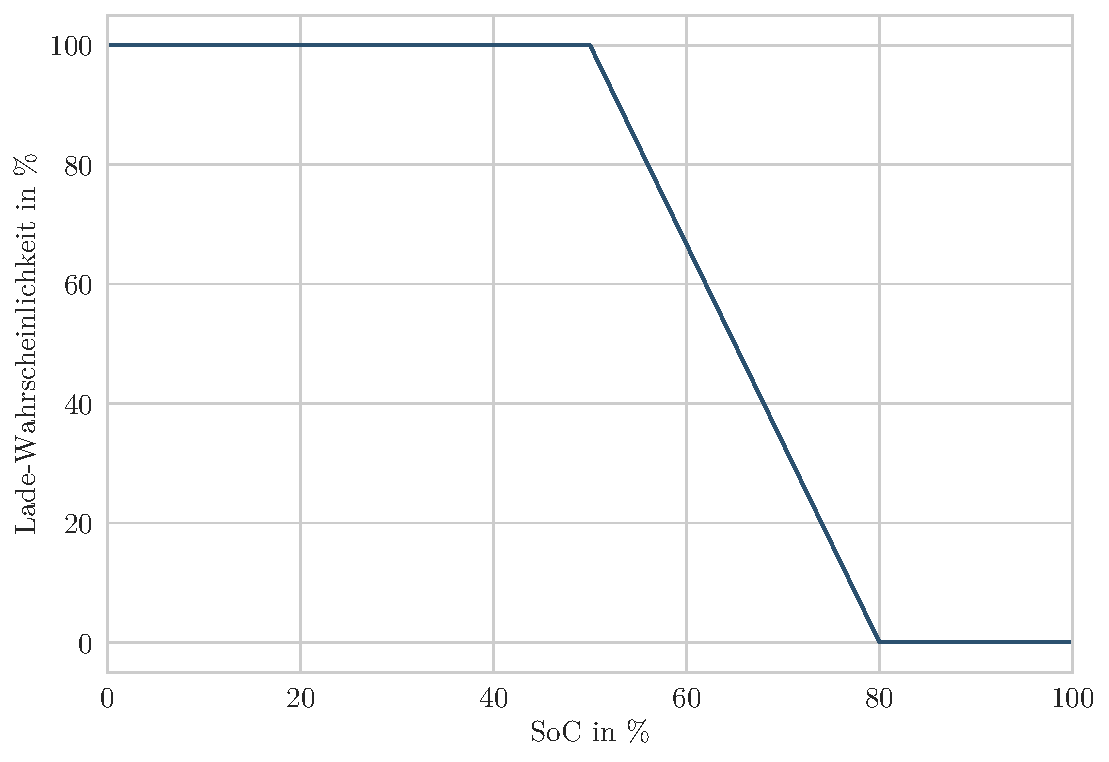
\includegraphics[width=\textwidth]{Bilder/soc_charging_prob}
    \caption{Abhängigkeit der Ladewahrscheinlichkeit vom SoC an öffentlichen Standorten}\label{fig:soc_charging_prob}
\end{figure}

Schnellladeinfrastruktur besitzt aufgrund des zusätzlichen Fahrt- und Zeitaufwandes eine geringe Attraktivität für den Nutzer.
Deshalb wird eine Schnellladung in dieser Simulation nur dann ausgelöst, wenn es wirklich nötig ist.
Sinkt der \gls{SOC} eines Fahrzeugs unter \SI{15}{\percent}, wird eine Schnellladestation angefahren und das Fahrzeug wird für \SI{15}{\Minuten} geladen.
Im Unterschied zu \glspl{BEV}, können \glspl{PHEV} auch mit einem \gls{SOC} von \SI{0}{\percent} ihre Fahrt mit Hilfe des Verbrennungsmotors fortsetzen.
Aus diesem Grund wird bei \glspl{PHEV} kein Schnellladevorgang ausgelöst.\medskip

\subsubsection{Regionalisierung}

Die Regionalisierung der Fahrzeuge auf die Landkreise findet auf Grundlage des Fahrzeugbestandes nach Zulassungsbezirken \cite[][Stand: \DTMdate{2020-01-01}]{KBAPLZ2020} statt.
Es wird davon ausgegangen, dass es zu keiner Verschiebung des Anteils am Bestand zwischen den Zulassungsbezirken kommt.
Dies bedeutet, dass die Gesamtanzahl der Fahrzeuge je Fahrzeugklasse je Szenario entsprechend des heutigen Bestandes anteilig verteilt wird.

\subsubsection{Implementierung der Ladestrategien in simbev}

Bereits ohne 

% TODO: Begründung warum eine kleineres Subset an Autos ausreicht, um auch größere Mengen von Fahrzeugen abzubilden

\subsubsection{Localiser Tool}

%\newpage

%\section{Einleitung}

\lipsum[24]

% You need inkscape for this
% inkscape needs to be in your PATH
\begin{figure}[H]
    \centering
    \includesvg[width=\textwidth]{Bilder/SurfPlot}
    \caption{Beispiel eines \texttt{Surface Plots} der drei Gleichungen des Gleichungssystems $A\vec{x} = \vec{b}$ nach $x_3$ aufgelöst}\label{fig:SurfPlot}
\end{figure}

In \autoref{fig:SurfPlot} findet sich ein Beispiel für eine \texttt{SVG}-Grafik. \lipsum[13]

\section{Theoretische Grundlagen}

\lipsum[32]

\begin{equation}
	E = \hbar \omega
	\label{eq:plancksrelation}
\end{equation}

\autoref{eq:plancksrelation} zeigt ein Beispiel für eine Gleichung. \lipsum

\section{Methodik}

\lipsum[27]

%{
\renewcommand{\arraystretch}{1.2}% grßerer Zeilenabstand
\sisetup{range-phrase=~{--}~}% Gedankenstrich statt "bis" bei SIrange
\begin{table}[H]
	\begin{center}
		\caption{Emissionsfaktoren von Biogasanlagen mit direkter Biogasverbrennung}
		\begin{tabu} to \textwidth {X X[1.5, r]}
			\hline
			Schadstoff	& Emissionen in \si[per-mode=symbol]{\mgkwh}					\\ \hline
			\ce{CO}		& \SIrange{922}{1116}{\relax}                               	\\
			\ce{SO2}	& \SI{90}{\relax}                                       		\\
			\ce{NO_X}	& \SIrange{727}{1944}{\relax}                               	\\
			\ce{NMVOC}	& \SIrange{36}{76}{\relax}                                  	\\
			\ce{CH2O}	& \SIrange{31}{50}{\relax}                                  	\\ \hline
			\multicolumn{2}{l}{Quellen: \cite{Paolini2018}}
		\end{tabu}
		\label{tab:tab_air-pollutants}
	\end{center}
	\vspace{-3mm}%Put here to reduce too much white space after your table
\end{table}
}

\autoref{tab:tab_air-pollutants} zeigt ein Beispiel für eine Tabelle. \lipsum

\section{Ergebnisse}

\lipsum[14]

\begin{code}
    \captionof{listing}{Gaußsches Eliminationsverfahren}\label{code:GaussElem}
    \begin{minted}[
		linenos=true,
		numbersep=-10pt,
		obeytabs=true,
		tabsize=4,
		]{matlab}
		%% Gaussian Elimination
		% bringing the Matrix into upper triangular form
		% initializing a new matrix to keep the previous results
		GaussMat = OrdMat;
		% and a new vector
		GaussVec = OrdVec;
		% for loop over m-1 elements
		for i = 1:m-1
		   % Calculating the Row Multiplier by dividing the
		   % i Element of the row i+1:m through the
		   % i,i Element of the matrix
		   Mult = GaussMat(i+1:m,i) / GaussMat(i,i);
		   % Calculating the new rows of the matrix
		   GaussMat(i+1:m,:) = GaussMat(i+1:m,:) - Mult*GaussMat(i,:);
		   % and the vector
		   GaussVec(i+1:m,:) = GaussVec(i+1:m,:) - Mult*GaussVec(i,:);
		end

		% removing rounding errors near zero
		threshold=10^(-12);
		% set near zeros to zero in the Matrix
		GaussMat(abs(GaussMat)<threshold) = 0;
		% set near zeros to zero in the Vector
		GaussVec(abs(GaussVec)<threshold) = 0;
		% initializing the solution vector x
		X = zeros(m,1);
		% determining the first element of the solution
		X(m,:) = GaussVec(m,:)/GaussMat(m,m);
		% for loop over the missing solutions
		for i = m-1:-1:1
		   % Calculating the i element of x by substracting product
		   % of the known elements of x and the corresponding row of
		   % the Gauss Matrix from the corresponding element of the
		   % Gauss Vector and dividing the outcome by
		   % the matrix element i,i
		   X(i,:) = ((GaussVec(i,:) -...
					GaussMat(i,i+1:m)*X(i+1:m,:))/GaussMat(i,i));
		end
	\end{minted}
\end{code}

Im \autoref{code:GaussElem} findet sich ein Beispiel für die Darstellung eines Codeblockes. \lipsum

\section{Diskussion}

\lipsum[18] Beispiel für die Darstellung von \texttt{SI}-Einheiten: \SIrange{1.20}{7.32}{\newton\per\square\meter}. \lipsum

\section{Fazit}

Hier findet sich ein Beispiel für eine Abkürzung: \gls{FEE}. Anschließend wird automatisch die Kurzform ausgegeben: \gls{FEE}. Um die Darstellung der Liste zu überprüfen, findet sich hier eine weitere Abkürzung im Plural: \glspl{EEG}. \lipsum~Ein weiteres Beispiel für eine Quelle mit Seitenzahl: \cite[][vgl. S. 12]{WIKUE2006}% Einige Beispiele

\newpage

%\begin{sloppypar}% erlaubt mehr whitespace, um URL's besser zu brechen
%	\printbibliography% Ausgabe der Literatur
%\end{sloppypar}%

\newpage

%\appendix

\section{Anhang}

\subsection{Daten der Metaanalyse}

{
\renewcommand{\arraystretch}{1.2}% grßerer Zeilenabstand
\sisetup{range-phrase=~{--}~}% Gedankenstrich statt "bis" bei SIrange
\begin{table}[H]
	\begin{center}
		\caption{Szenarienvergleich des Fahrzeugbestands von BEV bis zum Jahr \num{2050}}
		\begin{tabu} to \textwidth {X[5] X[1, r] X[1, r] X[1, r]}
			\hline
            Studie                                                                                          & \num{2030}     & \num{2040}     & \num{2050}     \\\hline
            \num{2014} {--} BMWi {--} Energiereferenzprognose \cite{PrognosAG2014}                          & \num{1755000}  & \num{3777000}  & \num{5514000}  \\
            \num{2014} {--} Öko{--}Institut e.V. {--} Grenzenlos \cite{Hacker2014}                          & \num{2000000}  & \num{16000000} & \num{29000000} \\
            \num{2014} {--} Öko{--}Institut e.V. {--} Regional \cite{Hacker2014}                            & \num{3000000}  & \num{11000000} & \num{15000000} \\
            \num{2014} {--} Shell {--} Alternativ \cite{Shell2014}                                          & \num{1200000}  & \num{3130000}  &                \\
            \num{2014} {--} Shell {--} Trend \cite{Shell2014}                                               & \num{730000}   & \num{1610000}  &                \\
            \num{2015} {--} DIW {--} BAU \cite{Schill2015}                                                  & \num{900000}   &                &                \\
            \num{2015} {--} DIW {--} EM\Plus~\cite{Schill2015}                                              & \num{1000000}  &                &                \\
            \num{2015} {--} Öko-Institut e.V. {--} KSZ {--} \SI{80}{\percent}-Pfad \cite{OekoInstitut2015}  &                &                & \num{19982000} \\
            \num{2015} {--} Öko-Institut e.V. {--} KSZ {--} \SI{95}{\percent}-Pfad \cite{OekoInstitut2015}  &                &                & \num{21619000} \\
            \num{2015} {--} Öko-Institut e.V. {--} KSZ {--} Referenz \cite{OekoInstitut2015}                &                &                & \num{3192000}  \\
            \num{2015} {--} SCelecTRA {--} konservativ \cite{Kanudia2016}                                   & \num{1060359}  &                &                \\
            \num{2015} {--} SCelecTRA {--} optimistisch \cite{Kanudia2016}                                  & \num{5197630}  &                &                \\
            \num{2016} {--} Renewbility {--} Basis \cite{Institut2016}                                      & \num{449000}   &                & \num{3203000}  \\
            \num{2016} {--} Renewbility {--} Effizienz \cite{Institut2016}                                  & \num{1001000}  &                & \num{17794000} \\
            \num{2016} {--} Renewbility {--} Effizienz-Plus \cite{Institut2016}                             & \num{1037000}  &                & \num{15452000} \\
            \num{2016} {--} TREMOD \cite{Knoerr2016}                                                        & \num{1960000}  &                &                \\
            \num{2016} {--} UBA {--} E\Plus~\cite{Kasten2016}                                               & \num{1629834}  & \num{11450915} & \num{23849848} \\
            \num{2016} {--} UBA {--} Fl\Plus~\cite{Kasten2016}                                              & \num{434355}   & \num{1341568}  & \num{2744870}  \\
            \num{2017} {--} BMWi {--} LFS {--} \SI{80}{\percent}-Pfad \cite{Pfluger2017}                    &                &                & \num{15500000} \\
            \num{2017} {--} BMWi {--} LFS {--} \SI{95}{\percent}-Pfad \cite{Pfluger2017}                    &                &                & \num{7200000}  \\
            \num{2017} {--} Öko-Institut e.V. \cite{Timpe2017}                                              & \num{1035900}  &                &                \\
            \num{2018} {--} BCG/prognos {--} \SI{80}{\percent}-Pfad \cite{BCG2018}                          & \num{4000000}  & \num{11000000} & \num{21000000} \\
            \num{2018} {--} BCG/prognos {--} \SI{95}{\percent}-Pfad \cite{BCG2018}                          & \num{4000000}  & \num{13000000} & \num{28000000} \\
            \num{2018} {--} BCG/prognos {--} Referenz \cite{BCG2018}                                        & \num{2000000}  & \num{5000000}  & \num{9000000}  \\
            \num{2018} {--} dena-Leitstudie {--} EL \cite{DEAGH2018}                                        & \num{13300000} &                & \num{30200000} \\
            \num{2018} {--} dena-Leitstudie {--} Referenz \cite{DEAGH2018}                                  & \num{1900000}  &                & \num{5300000}  \\
            \num{2018} {--} dena-Leitstudie {--} TM \cite{DEAGH2018}                                        & \num{5600000}  &                & \num{12100000} \\
            \num{2018} {--} NPE {--} konservativ \cite{NPE2018}                                             & \num{4200000}  &                &                \\
            \num{2018} {--} NPE {--} optimistisch \cite{NPE2018}                                            & \num{7000000}  &                &                \\
            \num{2019} {--} Dynamis fuEL \cite{Fattler2019}                                                 & \num{9457200}  & \num{24440400} & \num{27410400} \\
            \num{2020} {--} BNetzA {--} B \num{2040} \cite{BNetzA2020}                                      &                & \num{14100000} &                \\
            \num{2020} {--} NPM \cite{NPZMAVE2020}                                                          & \num{7231000}  &                &                \\\hline
            \multicolumn{4}{l}{Erweiterung der Metastudie des FfE e.V. \cite{Ebner2019}}
		\end{tabu}
		\label{tab:RampUpBEV}
	\end{center}
	\vspace{-3mm}%Put here to reduce too much white space after your table
\end{table}
}

{
\renewcommand{\arraystretch}{1.2}% grßerer Zeilenabstand
\sisetup{range-phrase=~{--}~}% Gedankenstrich statt "bis" bei SIrange
\begin{table}[H]
	\begin{center}
		\caption{Szenarienvergleich des Fahrzeugbestands von PHEV bis zum Jahr \num{2050}}
		\begin{tabu} to \textwidth {X[5] X[1, r] X[1, r] X[1, r]}
			\hline
            Studie                                                                                              & \num{2030}     & \num{2040}     & \num{2050}     \\\hline
            \num{2014} {--} BMWi {--} Energiereferenzprognose   \cite{PrognosAG2014}                            & \num{1084000}  & \num{2180000}  & \num{3298000}  \\
            \num{2014} {--} Öko-Institut e.V. {--} Grenzenlos   \cite{Hacker2014}                               & \num{2000000}  & \num{3000000}  & \num{3000000}  \\
            \num{2014} {--} Öko-Institut e.V. {--} Regional \cite{Hacker2014}                                   & \num{1000000}  & \num{2000000}  & \num{1000000}  \\
            \num{2014} {--} Shell {--} Alternativ \cite{Shell2014}                                              & \num{1920000}  & \num{5450000}  & \num{5500000}  \\
            \num{2014} {--} Shell {--} Trend \cite{Shell2014}                                                   & \num{1070000}  & \num{2620000}  &                \\
            \num{2015} {--} DIW {--} BAU \cite{Schill2015}                                                      & \num{2900000}  &                &                \\
            \num{2015} {--} DIW {--} EM\Plus~ \cite{Schill2015}                                                 & \num{3700000}  &                &                \\
            \num{2015} {--} Öko-Institut e.V. {--} KSZ {--}   \SI{80}{{\percent}}-Pfad \cite{OekoInstitut2015}  &                &                & \num{10301000} \\
            \num{2015} {--} Öko-Institut e.V. {--} KSZ {--} \SI{95}{{\percent}}-Pfad   \cite{OekoInstitut2015}  &                &                & \num{9178000}  \\
            \num{2015} {--} Öko-Institut e.V. {--} KSZ {--} Referenz   \cite{OekoInstitut2015}                  &                &                & \num{11995000} \\
            \num{2016} {--} Renewbility {--} Basis \cite{Institut2016}                                          & \num{2513000}  &                & \num{6478000}  \\
            \num{2016} {--} Renewbility {--} Effizienz   \cite{Institut2016}                                    & \num{5387000}  &                & \num{13928000} \\
            \num{2016} {--} Renewbility {--} Effizienz{--}Plus \cite{Institut2016}                              & \num{6485000}  &                & \num{13618000} \\
            \num{2016} {--} TREMOD \cite{Knoerr2016}                                                            & \num{3410000}  &                &                \\
            \num{2016} {--} UBA {--} E\Plus~ \cite{Kasten2016}                                                  & \num{7460315}  & \num{18418291} & \num{15562406} \\
            \num{2016} {--} UBA {--} Fl\Plus~ \cite{Kasten2016}                                                 & \num{5824650}  & \num{14965197} & \num{18409351} \\
            \num{2017} {--} BMWi {--} LFS {--} \SI{80}{{\percent}}-Pfad \cite{Pfluger2017}                      &                &                & \num{14600000} \\
            \num{2017} {--} BMWi {--} LFS {--}   \SI{95}{{\percent}}-Pfad \cite{Pfluger2017}                    &                &                & \num{8100000}  \\
            \num{2017} {--} Öko{--}Institut e.V. \cite{Timpe2017}                                               & \num{3798200}  &                &                \\
            \num{2018} {--} BCG/prognos {--}   \SI{80}{{\percent}}-Pfad \cite{BCG2018}                          & \num{6000000}  & \num{11000000} & \num{10000000} \\
            \num{2018} {--} BCG/prognos {--} \SI{95}{{\percent}}-Pfad \cite{BCG2018}                            & \num{6000000}  & \num{12000000} & \num{7000000}  \\
            \num{2018} {--} BCG/prognos {--} Referenz \cite{BCG2018}                                            & \num{7000000}  & \num{11000000} & \num{16000000} \\
            \num{2018} {--} dena-Leitstudie {--} EL \cite{DEAGH2018}                                            & \num{11000000} &                & \num{5600000}  \\
            \num{2018} {--} dena-Leitstudie {--} Referenz   \cite{DEAGH2018}                                    & \num{3200000}  &                & \num{6000000}  \\
            \num{2018} {--} dena-Leitstudie {--} TM \cite{DEAGH2018}                                            & \num{16400000} &                & \num{16000000} \\
            \num{2020} {--} NPM \cite{NPZMAVE2020}                                                              & \num{3259000}  &                &                \\\hline
            \multicolumn{4}{l}{Erweiterung der Metastudie des FfE e.V. \cite{Ebner2019}}
		\end{tabu}
		\label{tab:RampUpPHEV}
	\end{center}
	\vspace{-3mm}%Put here to reduce too much white space after your table
\end{table}
}

{
\renewcommand{\arraystretch}{1.2}% grßerer Zeilenabstand
\sisetup{range-phrase=~{--}~}% Gedankenstrich statt "bis" bei SIrange
\begin{table}[H]
	\begin{center}
		\caption{Bestand an Personenkraftwagen nach Segmenten am \DTMdate{2020-01-01} und Einteilung in Fahrzeugklassen}
		\begin{tabu} to \textwidth {X[1] X[1] X[1, r] X[1, r]}
            \hline
            Segment            & Klasse       & Anzahl         & Anteil              \\ \hline
            Kleinwagen         & Kleinwagen   & \num{8934345}  & \SI{18.7}{\percent} \\
            Minis              & Kleinwagen   & \num{3344523}  & \SI{7.0}{\percent}  \\
            Kompaktklasse      & Mittelklasse & \num{11983057} & \SI{25.1}{\percent} \\
            Mittelklasse       & Mittelklasse & \num{6286659}  & \SI{13.2}{\percent} \\
            Grossraum-Van      & Mittelklasse & \num{2024873}  & \SI{4.2}{\percent}  \\
            Mini-Van           & Mittelklasse & \num{1995789}  & \SI{4.2}{\percent}  \\
            Obere Mittelklasse & Mittelklasse & \num{1923514}  & \SI{4.0}{\percent}  \\
            Sonstige           & Mittelklasse & \num{1154183}  & \SI{2.4}{\percent}  \\
            SUVs               & Oberklasse   & \num{3765451}  & \SI{7.9}{\percent}  \\
            Geländewagen       & Oberklasse   & \num{2594849}  & \SI{5.4}{\percent}  \\
            Utilities          & Oberklasse   & \num{1931837}  & \SI{4.0}{\percent}  \\
            Sportwagen         & Oberklasse   & \num{918102}   & \SI{1.9}{\percent}  \\
            Wohnmobile         & Oberklasse   & \num{589354}   & \SI{1.2}{\percent}  \\
            Oberklasse         & Oberklasse   & \num{269441}   & \SI{.6}{\percent}   \\ \hline
            \multicolumn{4}{l}{Quelle: \cite{KBASegments2020}}
		\end{tabu}
		\label{tab:KBASegments}
	\end{center}
	\vspace{-3mm}%Put here to reduce too much white space after your table
\end{table}
}

{
\renewcommand{\arraystretch}{1.2}% grßerer Zeilenabstand
\sisetup{range-phrase=~{--}~}% Gedankenstrich statt "bis" bei SIrange
\begin{table}[H]
	\begin{center}
		\caption{Anteil der Fahrzeugklassen am Fahrzeugbestand am \DTMdate{2020-01-01}}
		\begin{tabu} to \textwidth {X[1] X[1, r]}
		    \hline
            Klasse       & Anteil              \\ \hline
            Kleinwagen   & \SI{25.7}{\percent} \\
            Mittelklasse & \SI{53.2}{\percent} \\
            Oberklasse   & \SI{21.1}{\percent} \\ \hline
            \multicolumn{2}{l}{Quelle: \cite{KBASegments2020}}
		\end{tabu}
		\label{tab:Segments}
	\end{center}
	\vspace{-3mm}%Put here to reduce too much white space after your table
\end{table}
}% Anhang

\end{document}